\documentclass[10pt,a4paper]{article}

% --- Essential Packages ---
\usepackage[utf8]{inputenc}
\usepackage[T1]{fontenc}
\usepackage{lmodern}
\usepackage[margin=0.62in,top=0.55in,bottom=0.55in]{geometry}
\usepackage{amsmath,amssymb,amsfonts,bm}
\usepackage{graphicx}
\usepackage{booktabs,tabularx,multirow,array}
\usepackage{xcolor}
\usepackage{fancyhdr}
\usepackage{titlesec}
\usepackage{microtype}
\usepackage{enumitem}
\usepackage{float}
\usepackage{tikz}
\usetikzlibrary{shapes.geometric, arrows.meta, positioning, calc, backgrounds, shadows}
\usepackage[colorlinks=true,linkcolor=navyblue,citecolor=tealblue,urlcolor=navyblue]{hyperref}

\usepackage{subcaption}
\captionsetup[subfigure]{font=small,labelfont=bf}

% --- Color Palette ---
\definecolor{navyblue}{RGB}{20, 45, 110}
\definecolor{tealblue}{RGB}{13, 148, 136}
\definecolor{accentpurple}{RGB}{124, 58, 237}
\definecolor{accentgreen}{RGB}{22, 163, 74}
\definecolor{darkslate}{RGB}{30, 41, 59}
\definecolor{amber}{RGB}{194, 65, 12}

% --- Page Header & Footer ---
\pagestyle{fancy}
\fancyhf{}
\fancyhead[L]{\small\sffamily\color{gray} MagMat $\cdot$ Physics-Grounded Screening}
\fancyhead[R]{\small\sffamily\color{gray} Sachin Poudel}
\fancyfoot[C]{\small\sffamily\color{darkslate}\thepage}
\renewcommand{\headrulewidth}{0.4pt}
\renewcommand{\footrulewidth}{0.0pt}

% --- Section Styling ---
\titleformat{\section}
  {\large\sffamily\bfseries\color{navyblue}}
  {\thesection}{0.5em}{}[\titlerule]
\titleformat{\subsection}
  {\normalsize\sffamily\bfseries\color{darkslate}}
  {\thesubsection}{0.4em}{}

\titlespacing*{\section}{0pt}{4pt}{2pt}
\titlespacing*{\subsection}{0pt}{2pt}{1pt}

\setlist{itemsep=0.5pt, topsep=1.0pt, parsep=0pt}
\setlength{\parskip}{1.2pt}
\setlength{\parindent}{10pt}

% Tight display math spacing
\setlength{\abovedisplayskip}{2.0pt}
\setlength{\belowdisplayskip}{2.0pt}
\setlength{\abovedisplayshortskip}{1pt}
\setlength{\belowdisplayshortskip}{1pt}

\begin{document}

% =========================================================================
% Page 1
% =========================================================================

% --- Simplified Title Block ---
\begin{center}
  {\Large\sffamily\bfseries\color{navyblue} MagMat: Physics-Grounded Screening for Permanent Magnets}\\[0.2em]
  {\large\sffamily Sachin Poudel}
\end{center}
\vspace{-0.6em}

\begin{abstract}
\noindent\small
Clean energy technologies such as electric vehicles and wind turbines depend heavily on high-performance permanent magnets, most of which require critical rare-earth elements with vulnerable supply chains. Accelerating the discovery of sustainable alternatives requires knowing what physics permits before training machine learning models. Here, we evaluate 56{,}781 experimental records against four classical condensed-matter boundaries: Slater-Pauling atomic band limits, Stoner quantum exchange, Kronmüller micromagnetics, and the Maxwell thermodynamic energy product ceiling. The results reveal a clear physical division: while saturation magnetization routinely nears its atomic band ceiling, measured coercivity achieves only $\approx$11\% of its theoretical single-crystal limit ($\alpha \approx 0.11$). This 89\% deficit originates in microstructural defects and grain boundary misalignment that chemical stoichiometry alone cannot describe. To bridge this reality gap, we combine 3D structural representations (DAO crystal diffusion and MACE equivariant transformers) with trained multi-task machine learning ensembles for magnetic phase classification and transition temperatures ($T_C, T_N$). An open-source interactive application enables real-time screening, physics boundary calculation, and inverse discovery for sustainable permanent magnets.
\end{abstract}
\vspace{-0.5em}

% =========================================================================
\section{Introduction and Workflow}
% =========================================================================
A permanent magnet has to do three things at once: hold a large magnetization, resist being demagnetized, and keep doing both while hot. Commercial magnets that manage this rely on Nd, Dy and Tb---the dependency that rare-earth-reduced candidates such as ordered FeNi (L1$_0$), $\tau$-MnAl and Fe$_{16}$N$_2$ are meant to break. Treating discovery as black-box fitting skips a cheaper step: classical upper bounds computable from stoichiometry alone establish what physics permits before machine learning is deployed (Figure~\ref{fig:workflow}).

\begin{figure}[H]
\centering
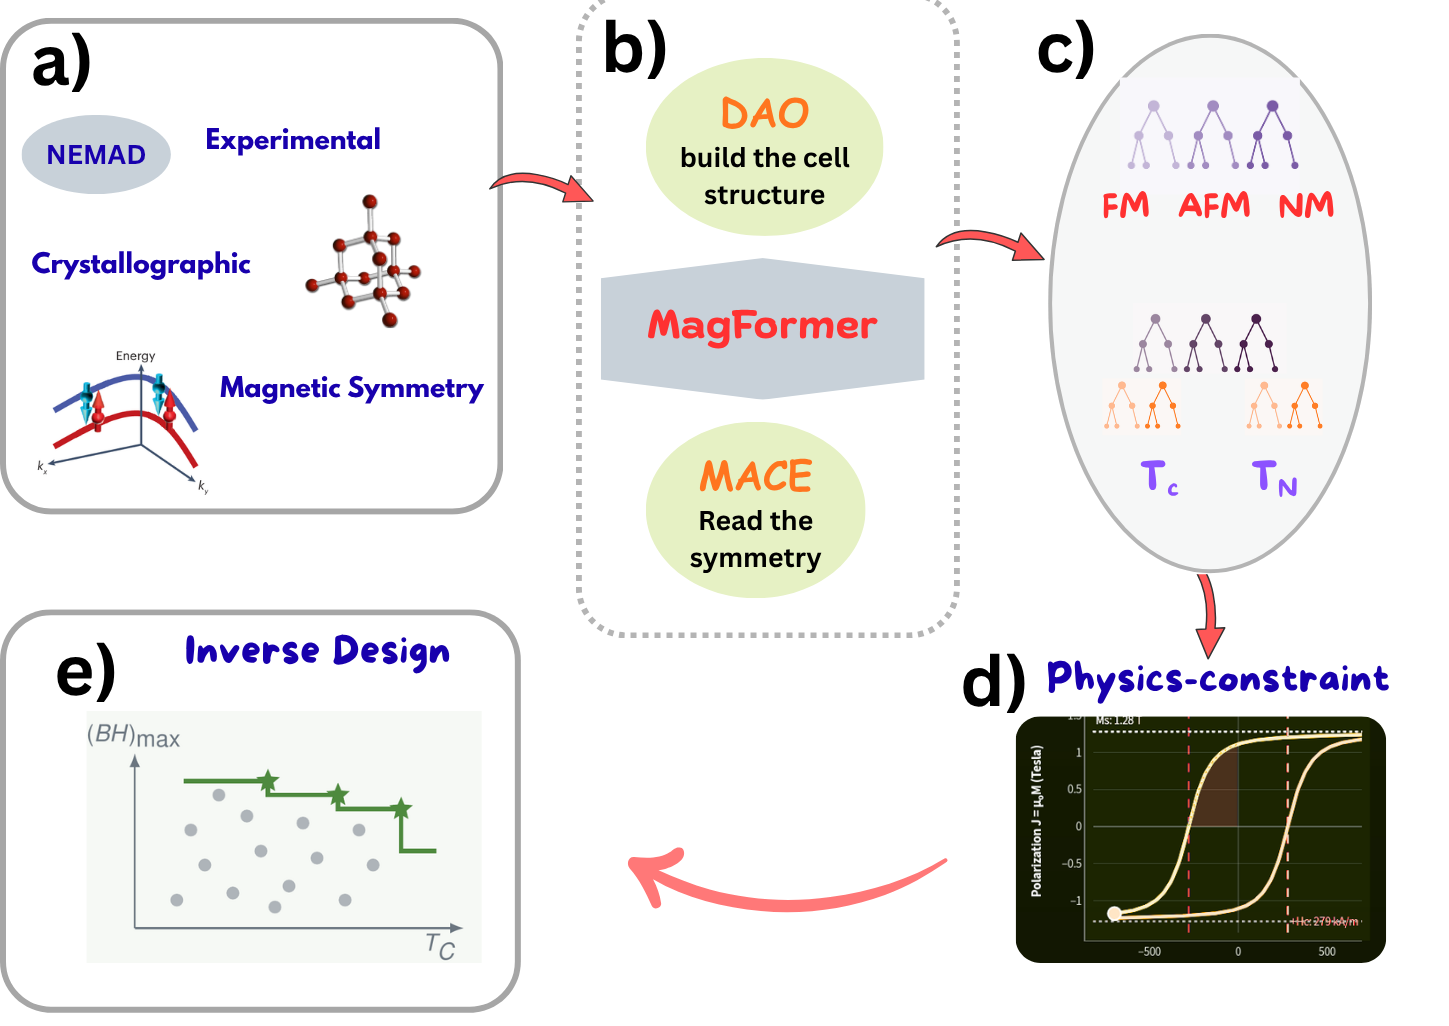
\includegraphics[height=6.4cm,keepaspectratio]{figures/methodology.png}
\vspace{-0.4em}
\caption{\footnotesize \textbf{Integrated screening and inverse-design workflow.} (a) Experimental datasets from NEMAD and literature with crystallographic and magnetic symmetry. (b) 3D foundation AI: DAO crystal diffusion (cell structure and $E_{\text{hull}}$ stability), MagFormer compositional transformer, and MACE equivariant symmetry. (c) Trained machine learning models: multi-model classifier for ground-state phase (FM, AFM, NM) and dynamic regression ensembles for transition temperatures ($T_C, T_N$). (d) Physics-constraint benchmarking against analytical condensed-matter ceilings (Kronmüller micromagnetics, Slater-Pauling, Maxwell bound). (e) Multi-objective inverse Pareto discovery ($(BH)_{\max}$ vs $T_C$).}
\label{fig:workflow}
\end{figure}
\vspace{-0.5em}

% =========================================================================
\section{Data Landscape and Target Coverage}
% =========================================================================
We harmonized 56,781 experimental records from the NIMS Electronic and Magnetic Alloy Database (NEMAD), Landolt-Börnstein handbooks and literature compilations, covering eight magnetic properties from intrinsic electronic parameters to extrinsic microstructural ones (Table~\ref{tab:dataset_summary}). Counts are restricted to physically plausible ranges.

\begin{table}[H]
\centering
\footnotesize
\renewcommand{\arraystretch}{0.88}
\caption{Harmonized experimental dataset coverage and summary statistics across eight magnetic targets.}
\label{tab:dataset_summary}
\vspace{0.1em}
\resizebox{\textwidth}{!}{%
\begin{tabular}{llrrrrrrr}
\toprule
\textbf{Target Property} & \textbf{Unit} & \textbf{Records} & \textbf{Coverage (\%)} & \textbf{Mean} & \textbf{Median} & \textbf{Std Dev} & \textbf{Range [Min, Max]} & \textbf{RE-Free Count} \\
\midrule
Curie Temp. ($T_C$) & K & 18,860 & 33.2\% & 373.5 & 323.0 & 276.3 & [1.0, 1500.0] & 8,572 (45.5\%) \\
Néel Temp. ($T_N$) & K & 7,734 & 13.6\% & 124.5 & 40.0 & 173.6 & [1.0, 1070.0] & 3,124 (40.4\%) \\
Saturation Mag. ($M_s$) & emu/g & 10,131 & 17.8\% & 60.0 & 44.8 & 60.8 & [0.01, 345.9] & 7,232 (71.4\%) \\
Coercivity ($H_c$) & A/m & 9,935 & 17.5\% & $4.58\times 10^5$ & $4.22\times 10^4$ & $2.06\times 10^6$ & [1.0, $9.55\times 10^7$] & 6,486 (65.3\%) \\
Anisotropy Const. ($K_1$) & J/m$^3$ & 4,582 & 8.1\% & $8.23\times 10^5$ & $4.80\times 10^3$ & $3.98\times 10^6$ & [$-7.2\times 10^7$, $8.8\times 10^7$] & 3,307 (72.2\%) \\
Max Energy Product ($(BH)_{\max}$) & kJ/m$^3$ & 1,658 & 2.9\% & 176.3 & 138.5 & 134.4 & [0.8, 647.8] & 571 (34.4\%) \\
Paramagnetic Curie ($\theta_p$) & K & 6,974 & 12.3\% & 29.4 & 1.0 & 181.8 & [$-991.0$, 1326.0] & 2,203 (31.6\%) \\
\bottomrule
\end{tabular}%
}
\end{table}
\vspace{-0.3em}

\noindent Two features matter downstream: coverage is \textbf{strongly asymmetric}---$(BH)_{\max}$ appears in under 3\% of records, while intrinsic quantities are far better sampled---and \textbf{dynamic ranges are wide}, with coercivity spanning eight decades, handled logarithmically.

\clearpage
% =========================================================================
% Page 2
% =========================================================================

\begin{figure}[t]
\centering
\begin{subfigure}[b]{0.485\textwidth}
  \centering
  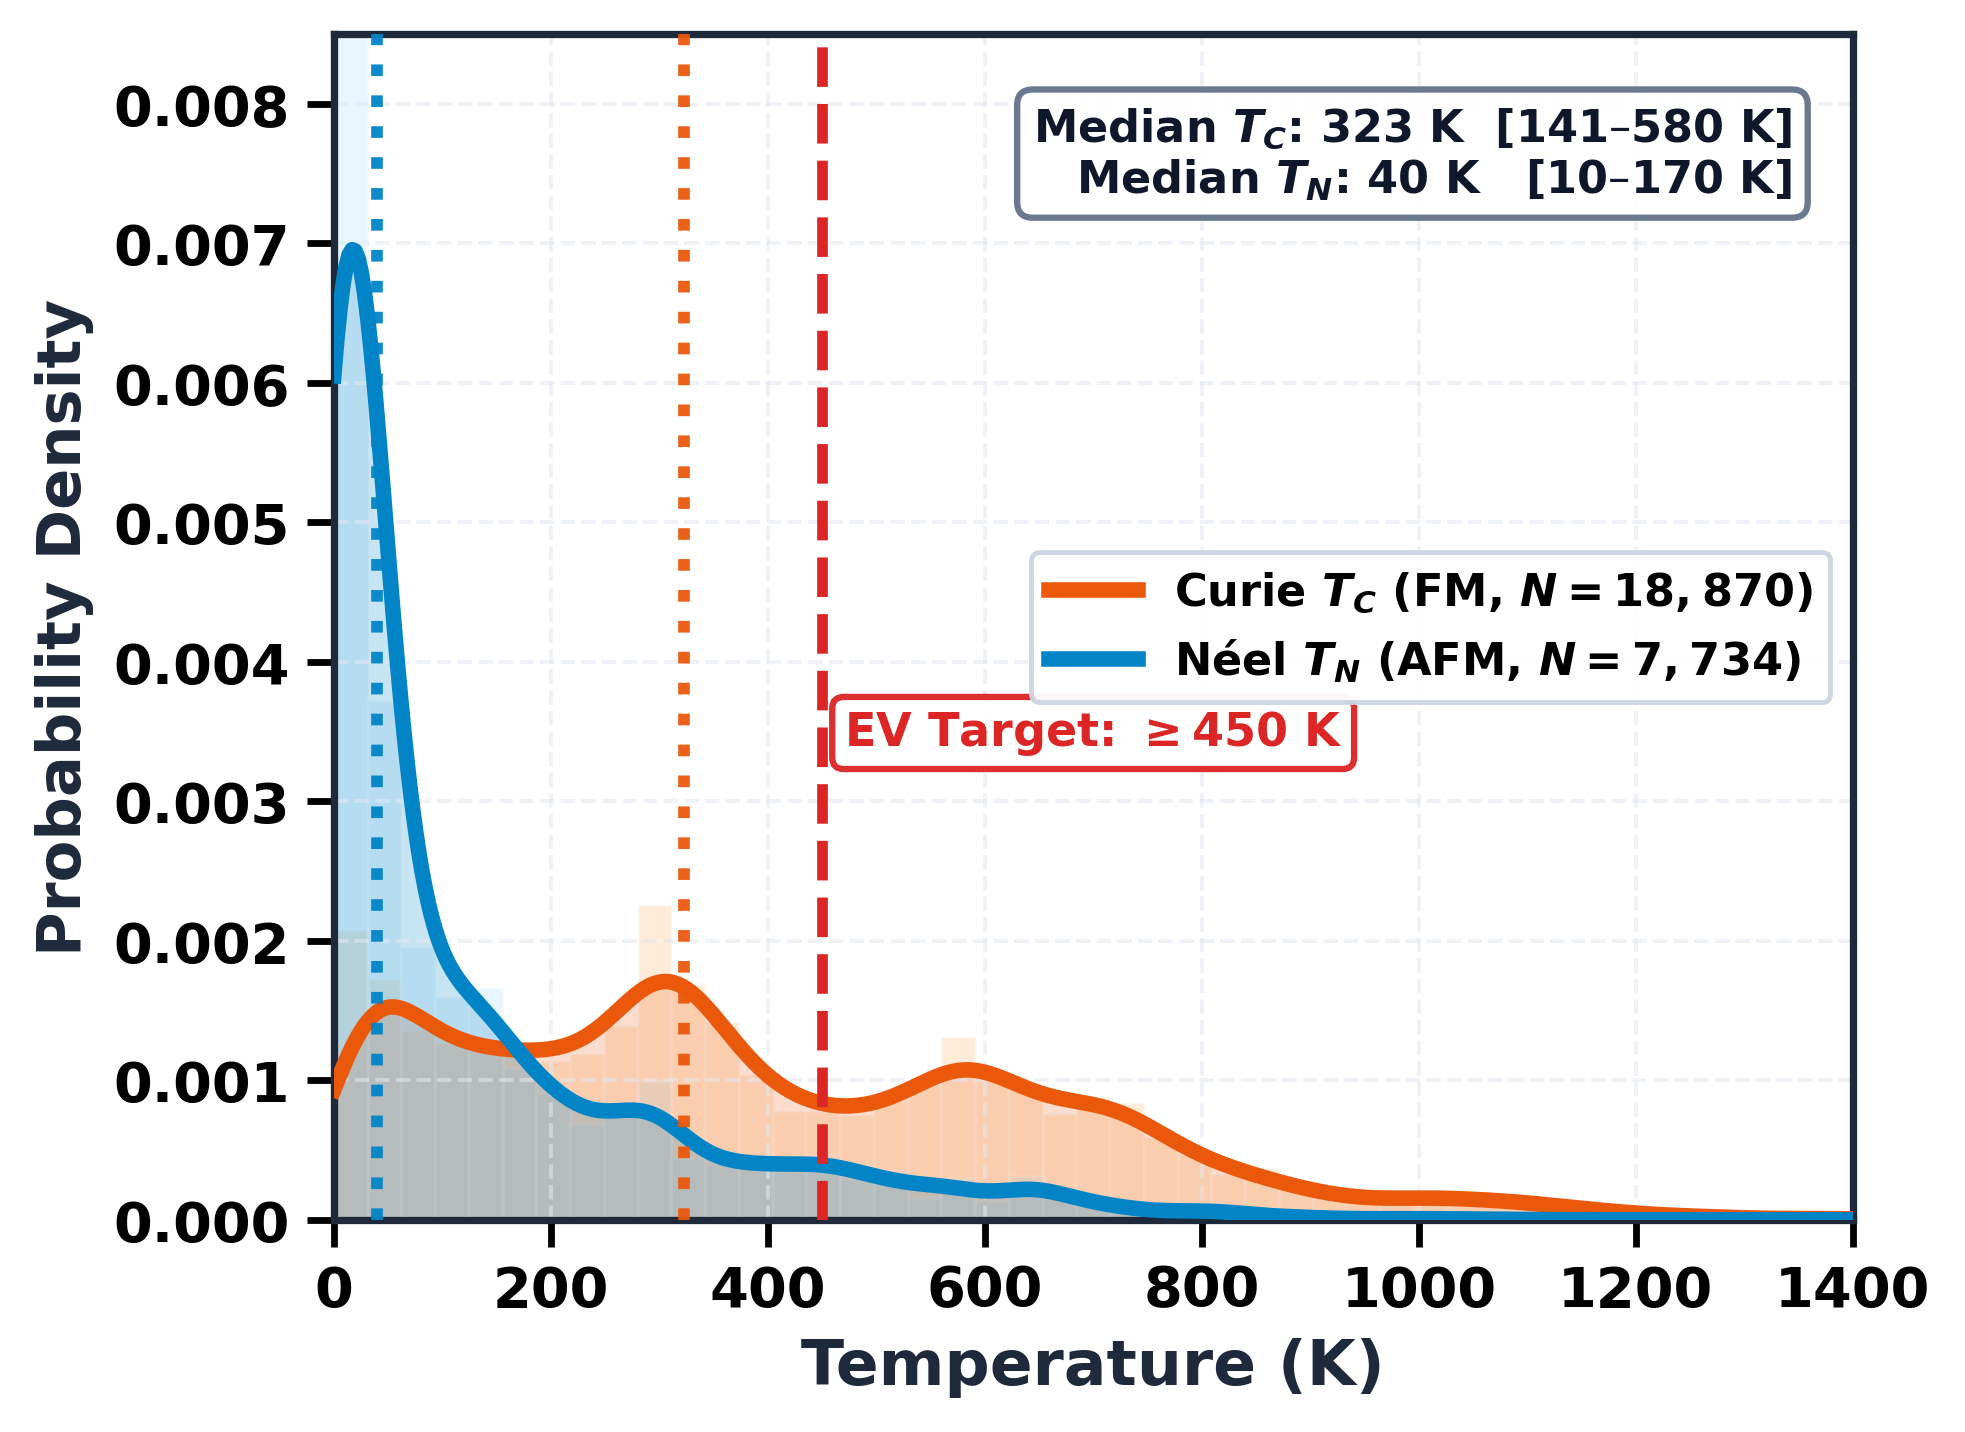
\includegraphics[height=3.35cm,keepaspectratio]{figures/dist_tc_tn.png}
  \caption{$T_C$ and $T_N$}
  \label{subfig:dist_tc_tn}
\end{subfigure}\hfill
\begin{subfigure}[b]{0.485\textwidth}
  \centering
  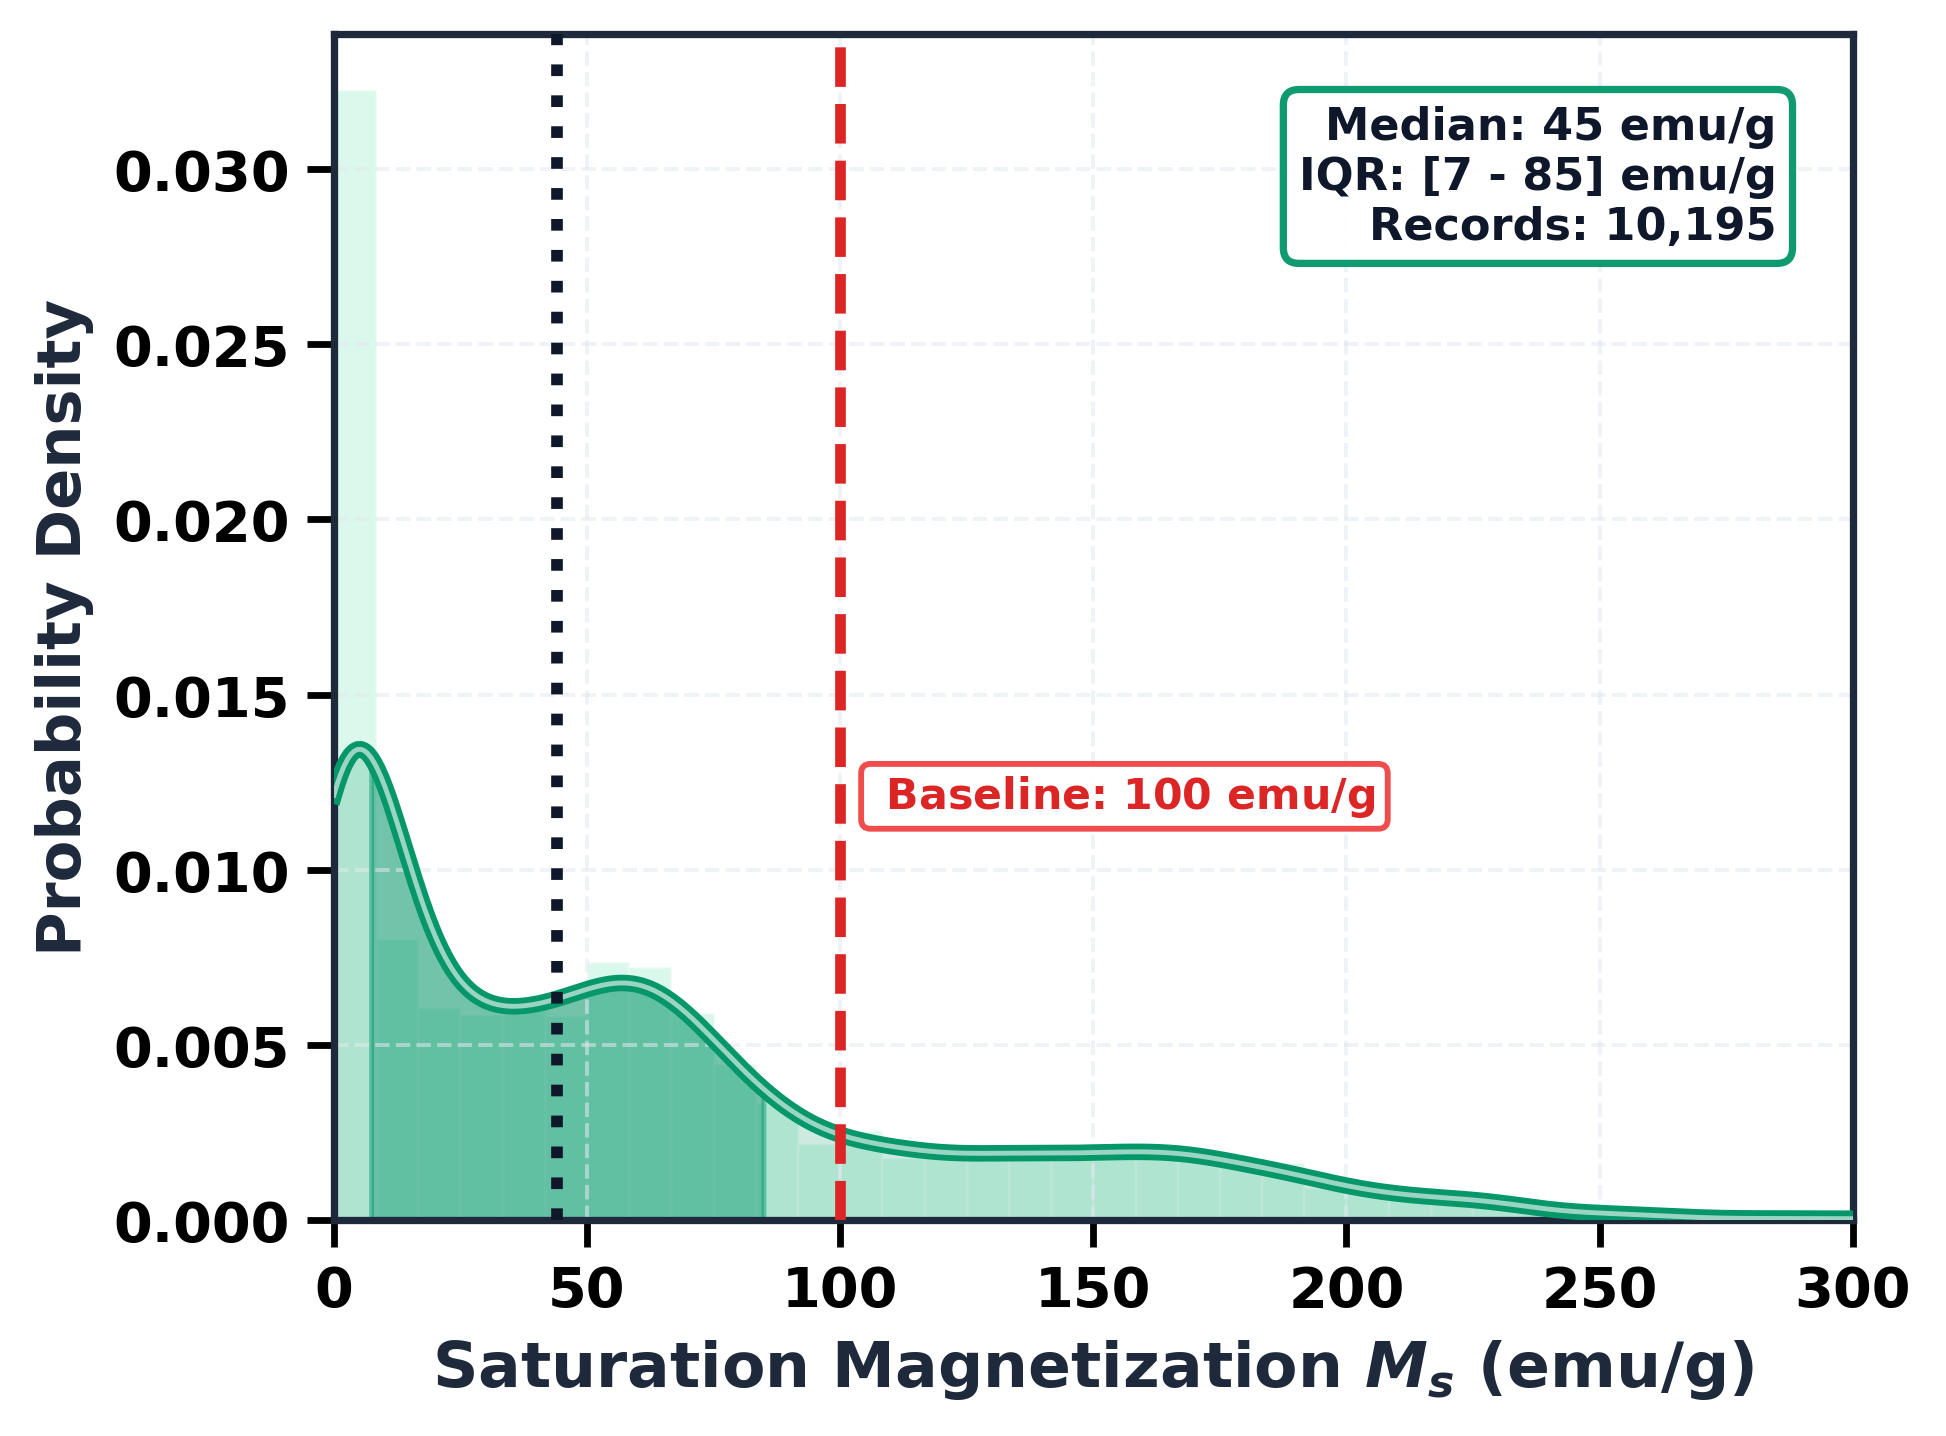
\includegraphics[height=3.35cm,keepaspectratio]{figures/dist_ms.png}
  \caption{$M_s$}
  \label{subfig:dist_ms}
\end{subfigure}\\[1pt]
\begin{subfigure}[b]{0.485\textwidth}
  \centering
  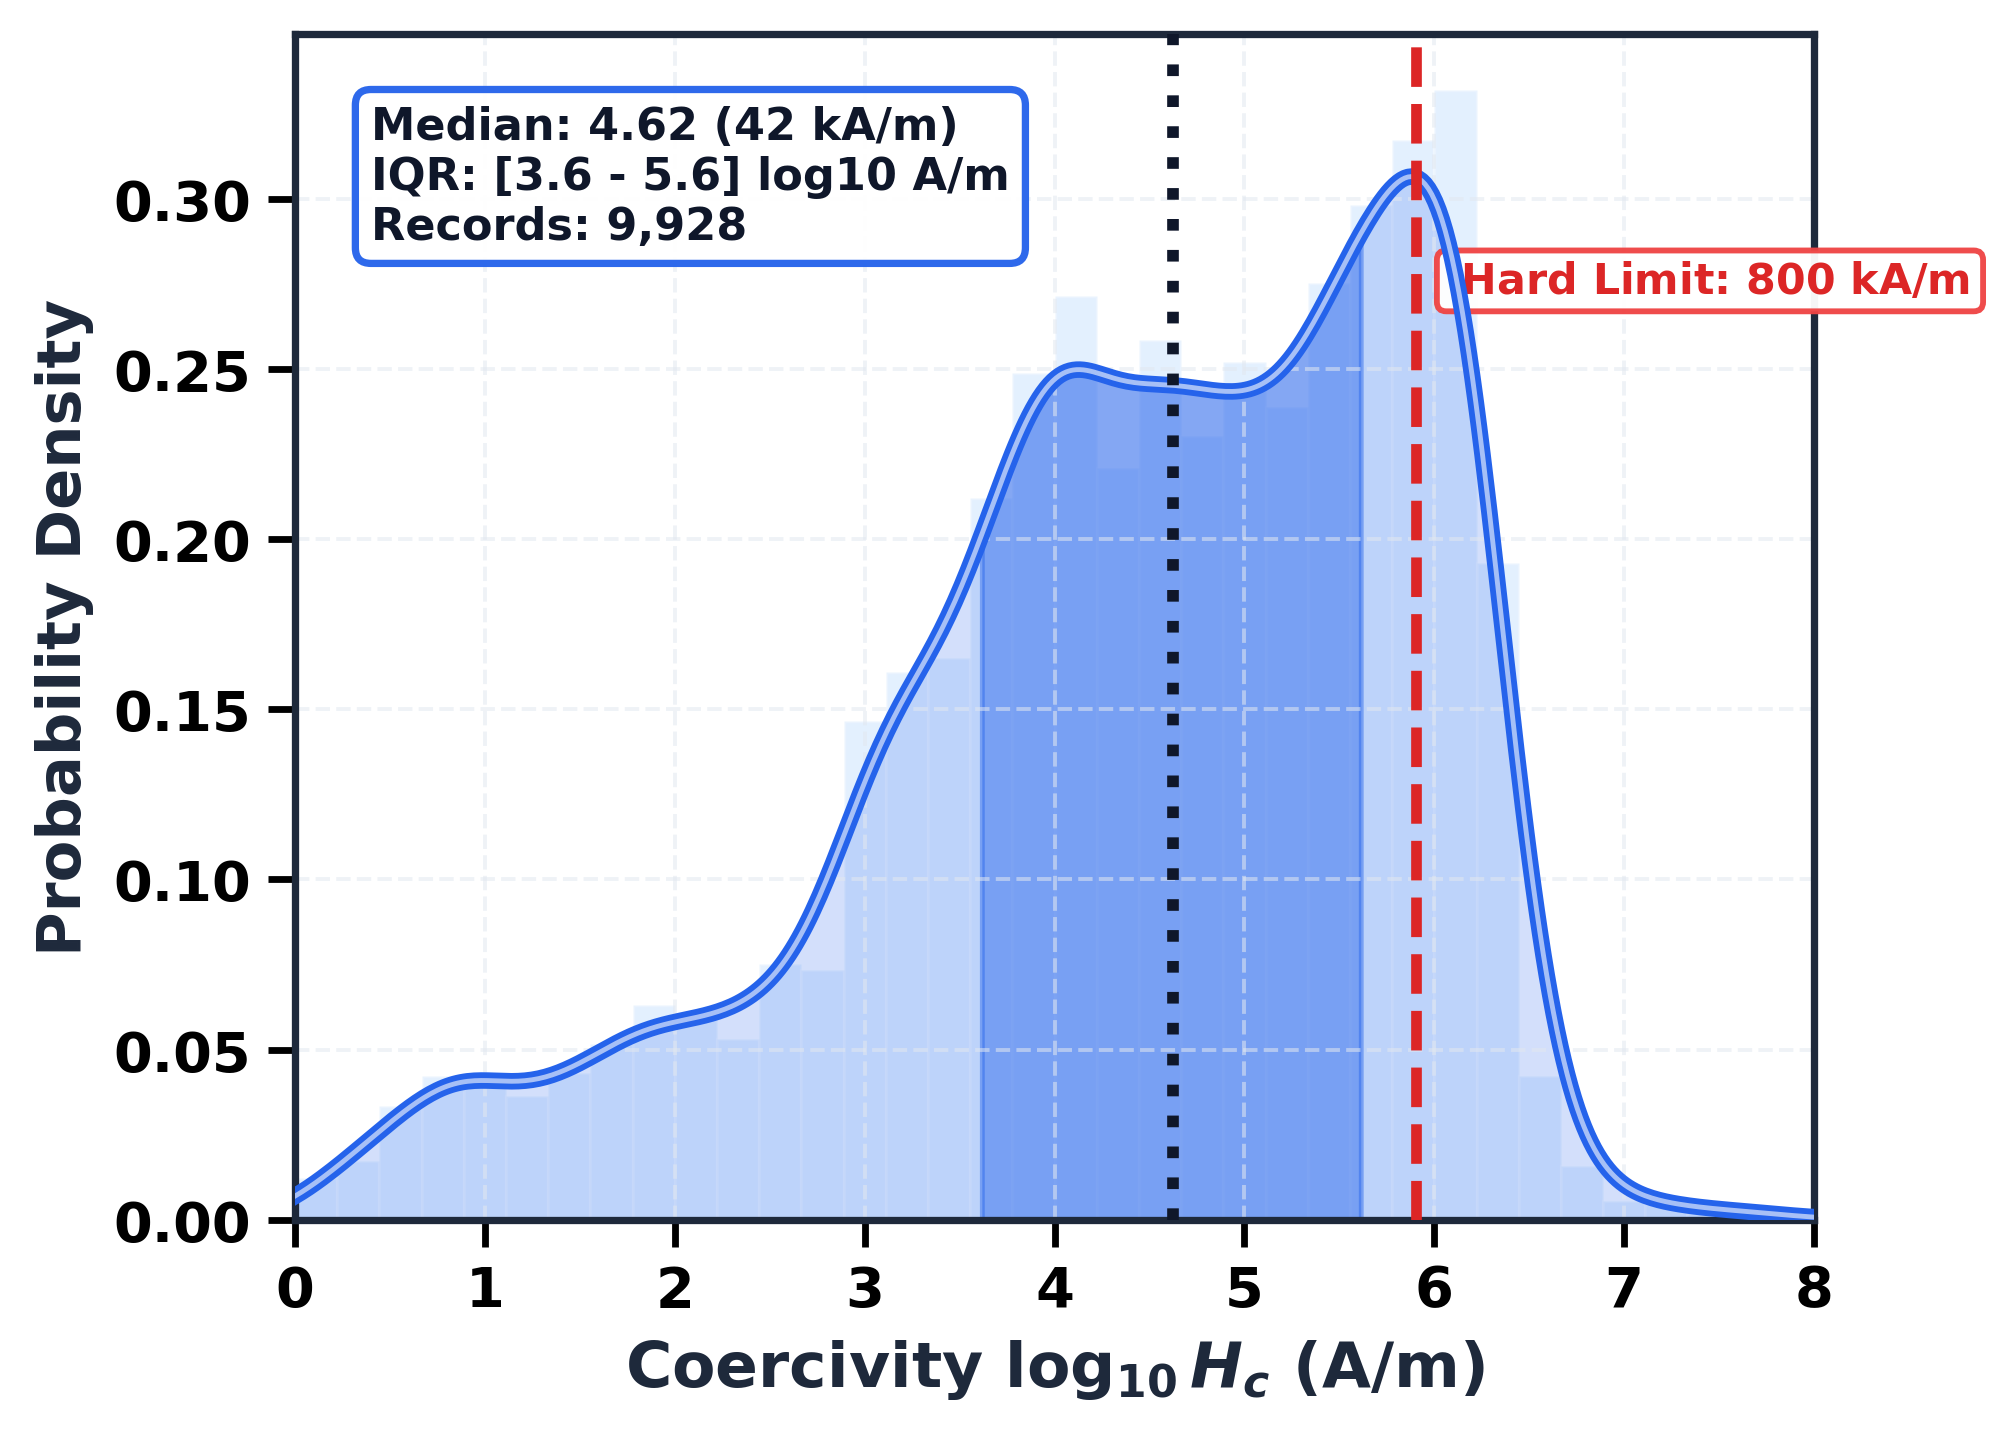
\includegraphics[height=3.35cm,keepaspectratio]{figures/dist_hc.png}
  \caption{$H_c$}
  \label{subfig:dist_hc}
\end{subfigure}\hfill
\begin{subfigure}[b]{0.485\textwidth}
  \centering
  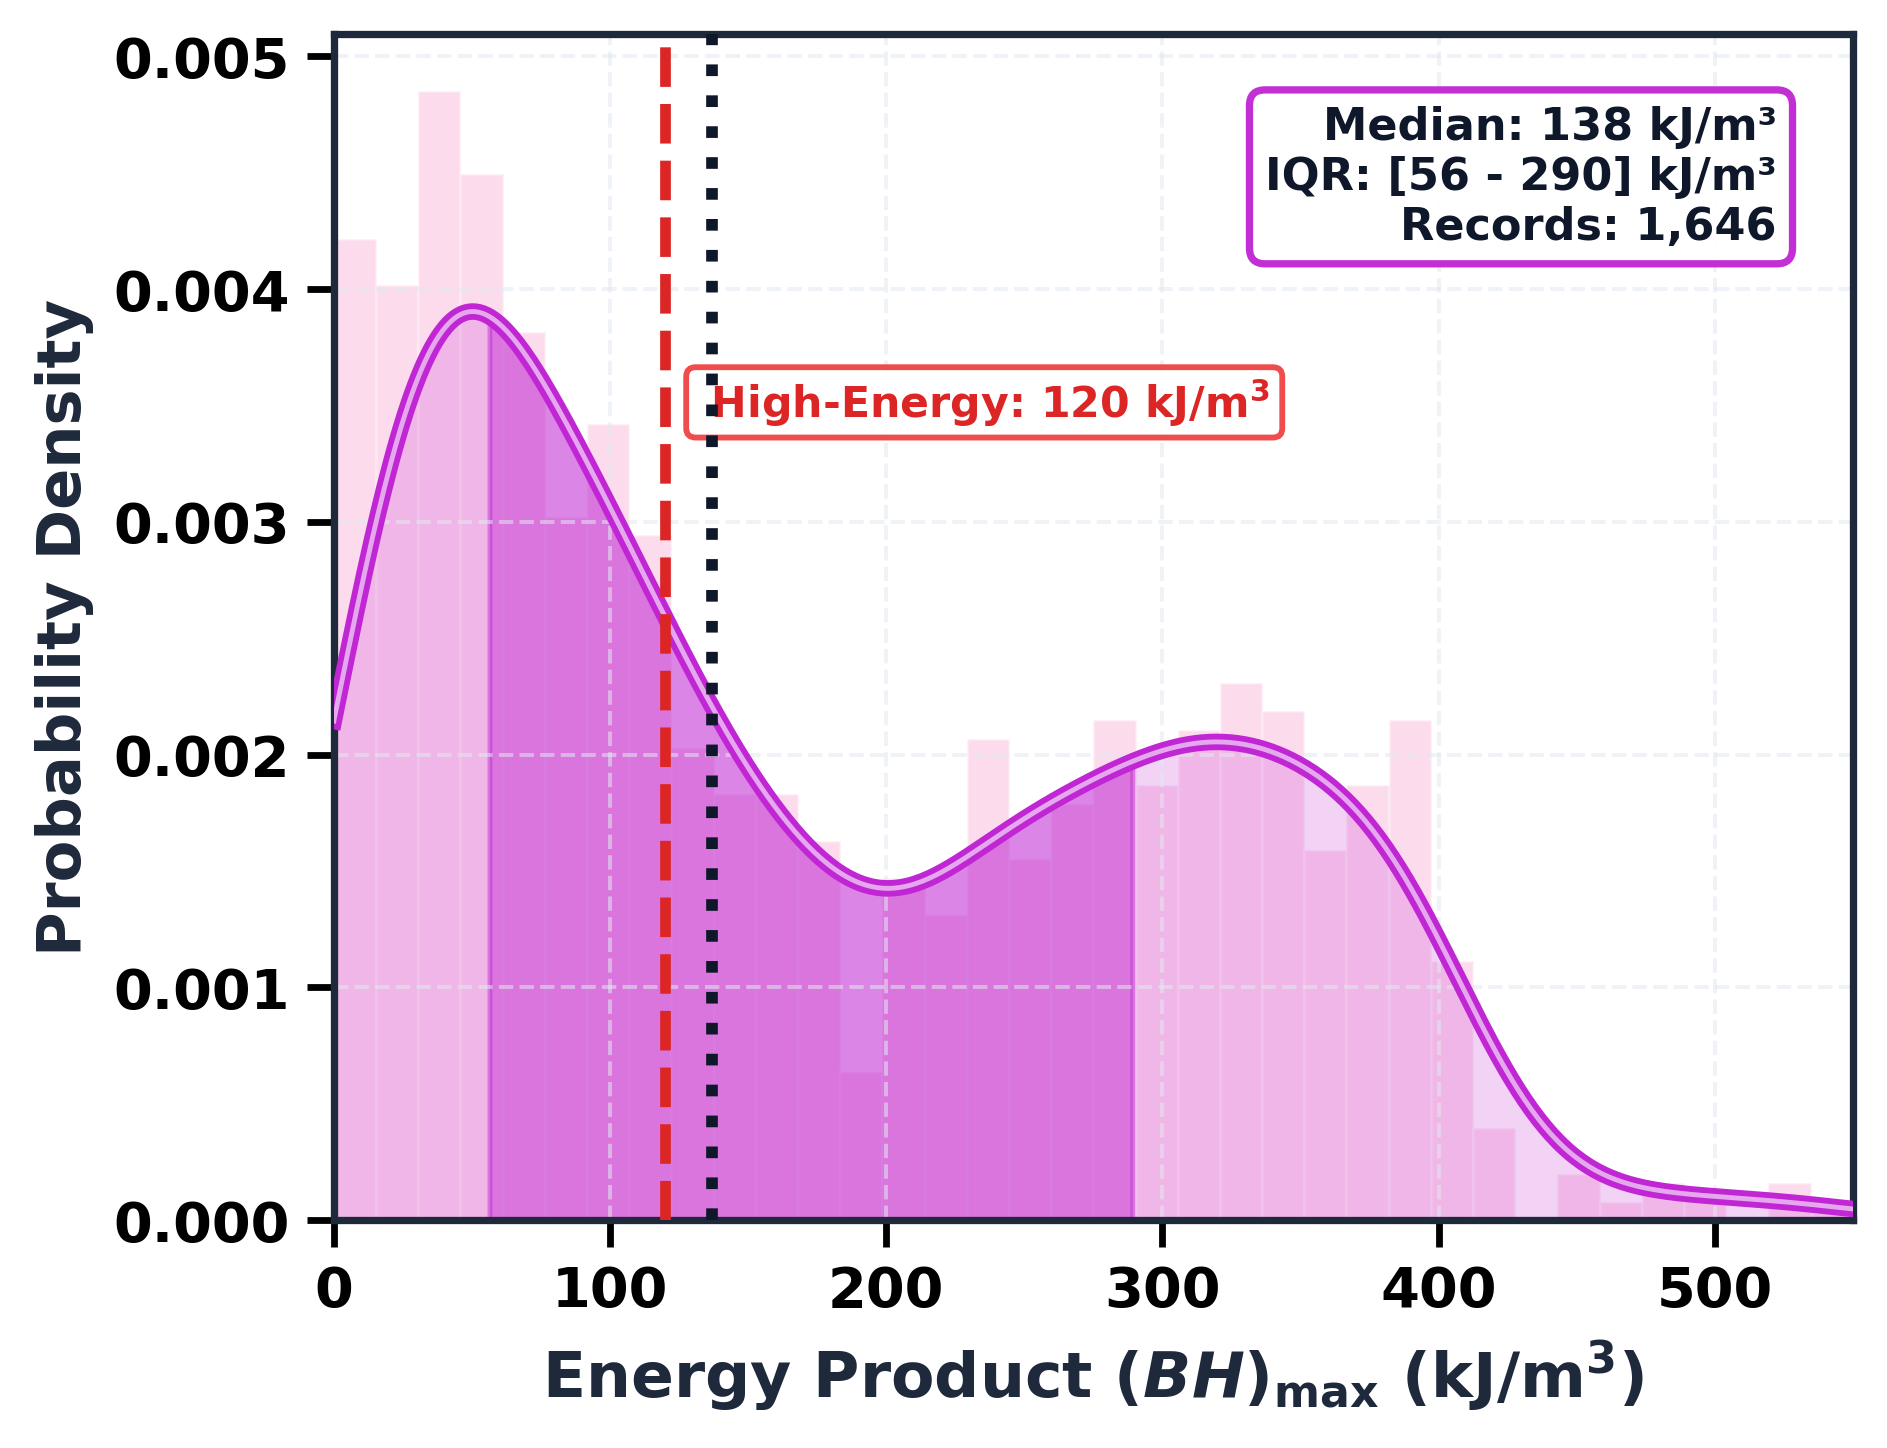
\includegraphics[height=3.35cm,keepaspectratio]{figures/dist_bhmax.png}
  \caption{$(BH)_{\max}$}
  \label{subfig:dist_bhmax}
\end{subfigure}
\vspace{-0.6em}
\caption{Empirical distributions for primary magnetic performance metrics: (a) transition temperatures ($T_C$ and $T_N$), (b) saturation magnetization $M_s$, (c) coercive field $\log_{10} H_c$, and (d) maximum energy product $(BH)_{\max}$.}
\label{fig:distributions}
\end{figure}
\vspace{-0.6em}

% =========================================================================
\section{Domain-Physics Baselines and Theoretical Ceilings}
% =========================================================================
Alongside trained empirical models, we benchmark experimental materials against four classical condensed-matter rules that establish theoretical performance bounds directly from composition and crystal physics without parameter fitting:

\noindent\textbf{Atomic Band Magnetization Ceiling (Slater-Pauling):} Magnetization in $3d$ alloys is governed by spin-polarized band filling. Valence electrons occupy majority-spin states up to $N_v \approx 8.3$, where the moment reaches its peak at $2.45\,\mu_B$/atom in Fe--Co, before falling as minority states fill:
\begin{equation}
\bar{\mu}_s = 
\begin{cases} 
2.45 - 0.875\,(8.3 - N_v) & (5.5 \le N_v < 8.3) \\
10.7 - N_v & (N_v \ge 8.3)
\end{cases},
\qquad M_s^{\text{SP}} = \frac{5585\,\bar{\mu}_s}{\bar{M}_{\text{mol}}} \quad [\text{emu/g}].
\end{equation}
Here $\bar{M}_{\text{mol}}$ is the mean atomic mass. Because both branches are anchored to elemental Fe, Co, and Ni, the ceiling is uniquely determined by stoichiometry.

\noindent\textbf{Exchange Coupling and Spontaneous Ordering (Stoner):} Spontaneous ferromagnetic ordering requires intra-atomic exchange to overcome the kinetic cost of band polarization, $I \cdot D(E_F) > 1$. While the local density of states $D(E_F)$ requires DFT, composition alone yields an effective ordering propensity based on transition-metal fraction and distance from the optimal valence concentration.

\noindent\textbf{Theoretical Nucleation Limit (Kronmüller Micromagnetics):} In an ideal defect-free crystal, coherent rotation against magnetocrystalline anisotropy $K_1$ establishes the nucleation ceiling $H_K = 2K_1 / \mu_0 M_s$. In real polycrystals, misoriented grain boundaries and localized defects trigger reverse domains prematurely, captured by the realization factor $\alpha$:
\begin{equation}
H_c \le H_K = \frac{2K_1}{\mu_0 M_s} \quad [\text{A/m}], \qquad \alpha = \frac{H_c}{H_K}.
\end{equation}
Across our harmonized database, the median realization factor is $\alpha \approx 0.11$, revealing an 89\% shortfall against theoretical single-crystal potential.

\noindent\textbf{Thermodynamic Energy Ceiling (Maxwell Limit):} For an ideal rectangular hysteresis loop with remanence $B_r = \mu_0 M_s$, magnetostatic energy density is strictly bounded by:
\begin{equation}
(BH)_{\max} \le \frac{1}{4} \mu_0 M_s^2 \quad [\text{kJ/m}^3].
\end{equation}
This thermodynamic ceiling cannot be exceeded by any processing method, providing an automated integrity check that flags inconsistent measurements.

\begin{table}[H]
\centering
\small
\renewcommand{\arraystretch}{0.84}
\caption{Quantitative evaluation of analytical physical ceilings across experimental test subsets without parameter fitting.}
\label{tab:baselines}
\vspace{0.1em}
\resizebox{\textwidth}{!}{%
\begin{tabular}{lllll}
\toprule
\textbf{Physical Model} & \textbf{Target Property} & \textbf{Evaluation Subset} & \textbf{Baseline Metric} & \textbf{Physical Mechanism Captured} \\
\midrule
Slater-Pauling Model & Saturation Mag. ($M_s$) & All Alloys ($n = 9,746$) & MAE = 87.4 emu/g ($r = 0.145$) & Average valence band filling \\
Slater-Pauling Model & Saturation Mag. ($M_s$) & $3d$-Rich Alloys ($n = 3,591$) & MAE = 79.6 emu/g ($r = 0.208$) & Majority/minority sub-band splitting \\
Thermodynamic Upper Bound & Energy Product ($(BH)_{\max}$) & Matched $M_s$--$(BH)_{\max}$ ($n = 498$) & \textbf{71.7\% within bound} & Maxwell energy density limit ($\frac{1}{4}\mu_0 M_s^2$) \\
Kronmüller Micromagnetics & Coercivity ($H_c$) & Matched $K_1$--$M_s$--$H_c$ ($n = 1,064$) & \textbf{Median $\alpha = 0.11$} (89\% shortfall) & Nucleation limit ($2K_1/\mu_0 M_s$) vs defect pinning \\
\bottomrule
\end{tabular}%
}
\end{table}

\clearpage
% =========================================================================
% Page 3
% =========================================================================

% =========================================================================
\section{Empirical Validation and Correlation Analysis}
% =========================================================================
Benchmarked against the four bounds, the experimental data reveals both where the ceilings bind and which descriptors drive which property.

\begin{figure}[t]
\centering
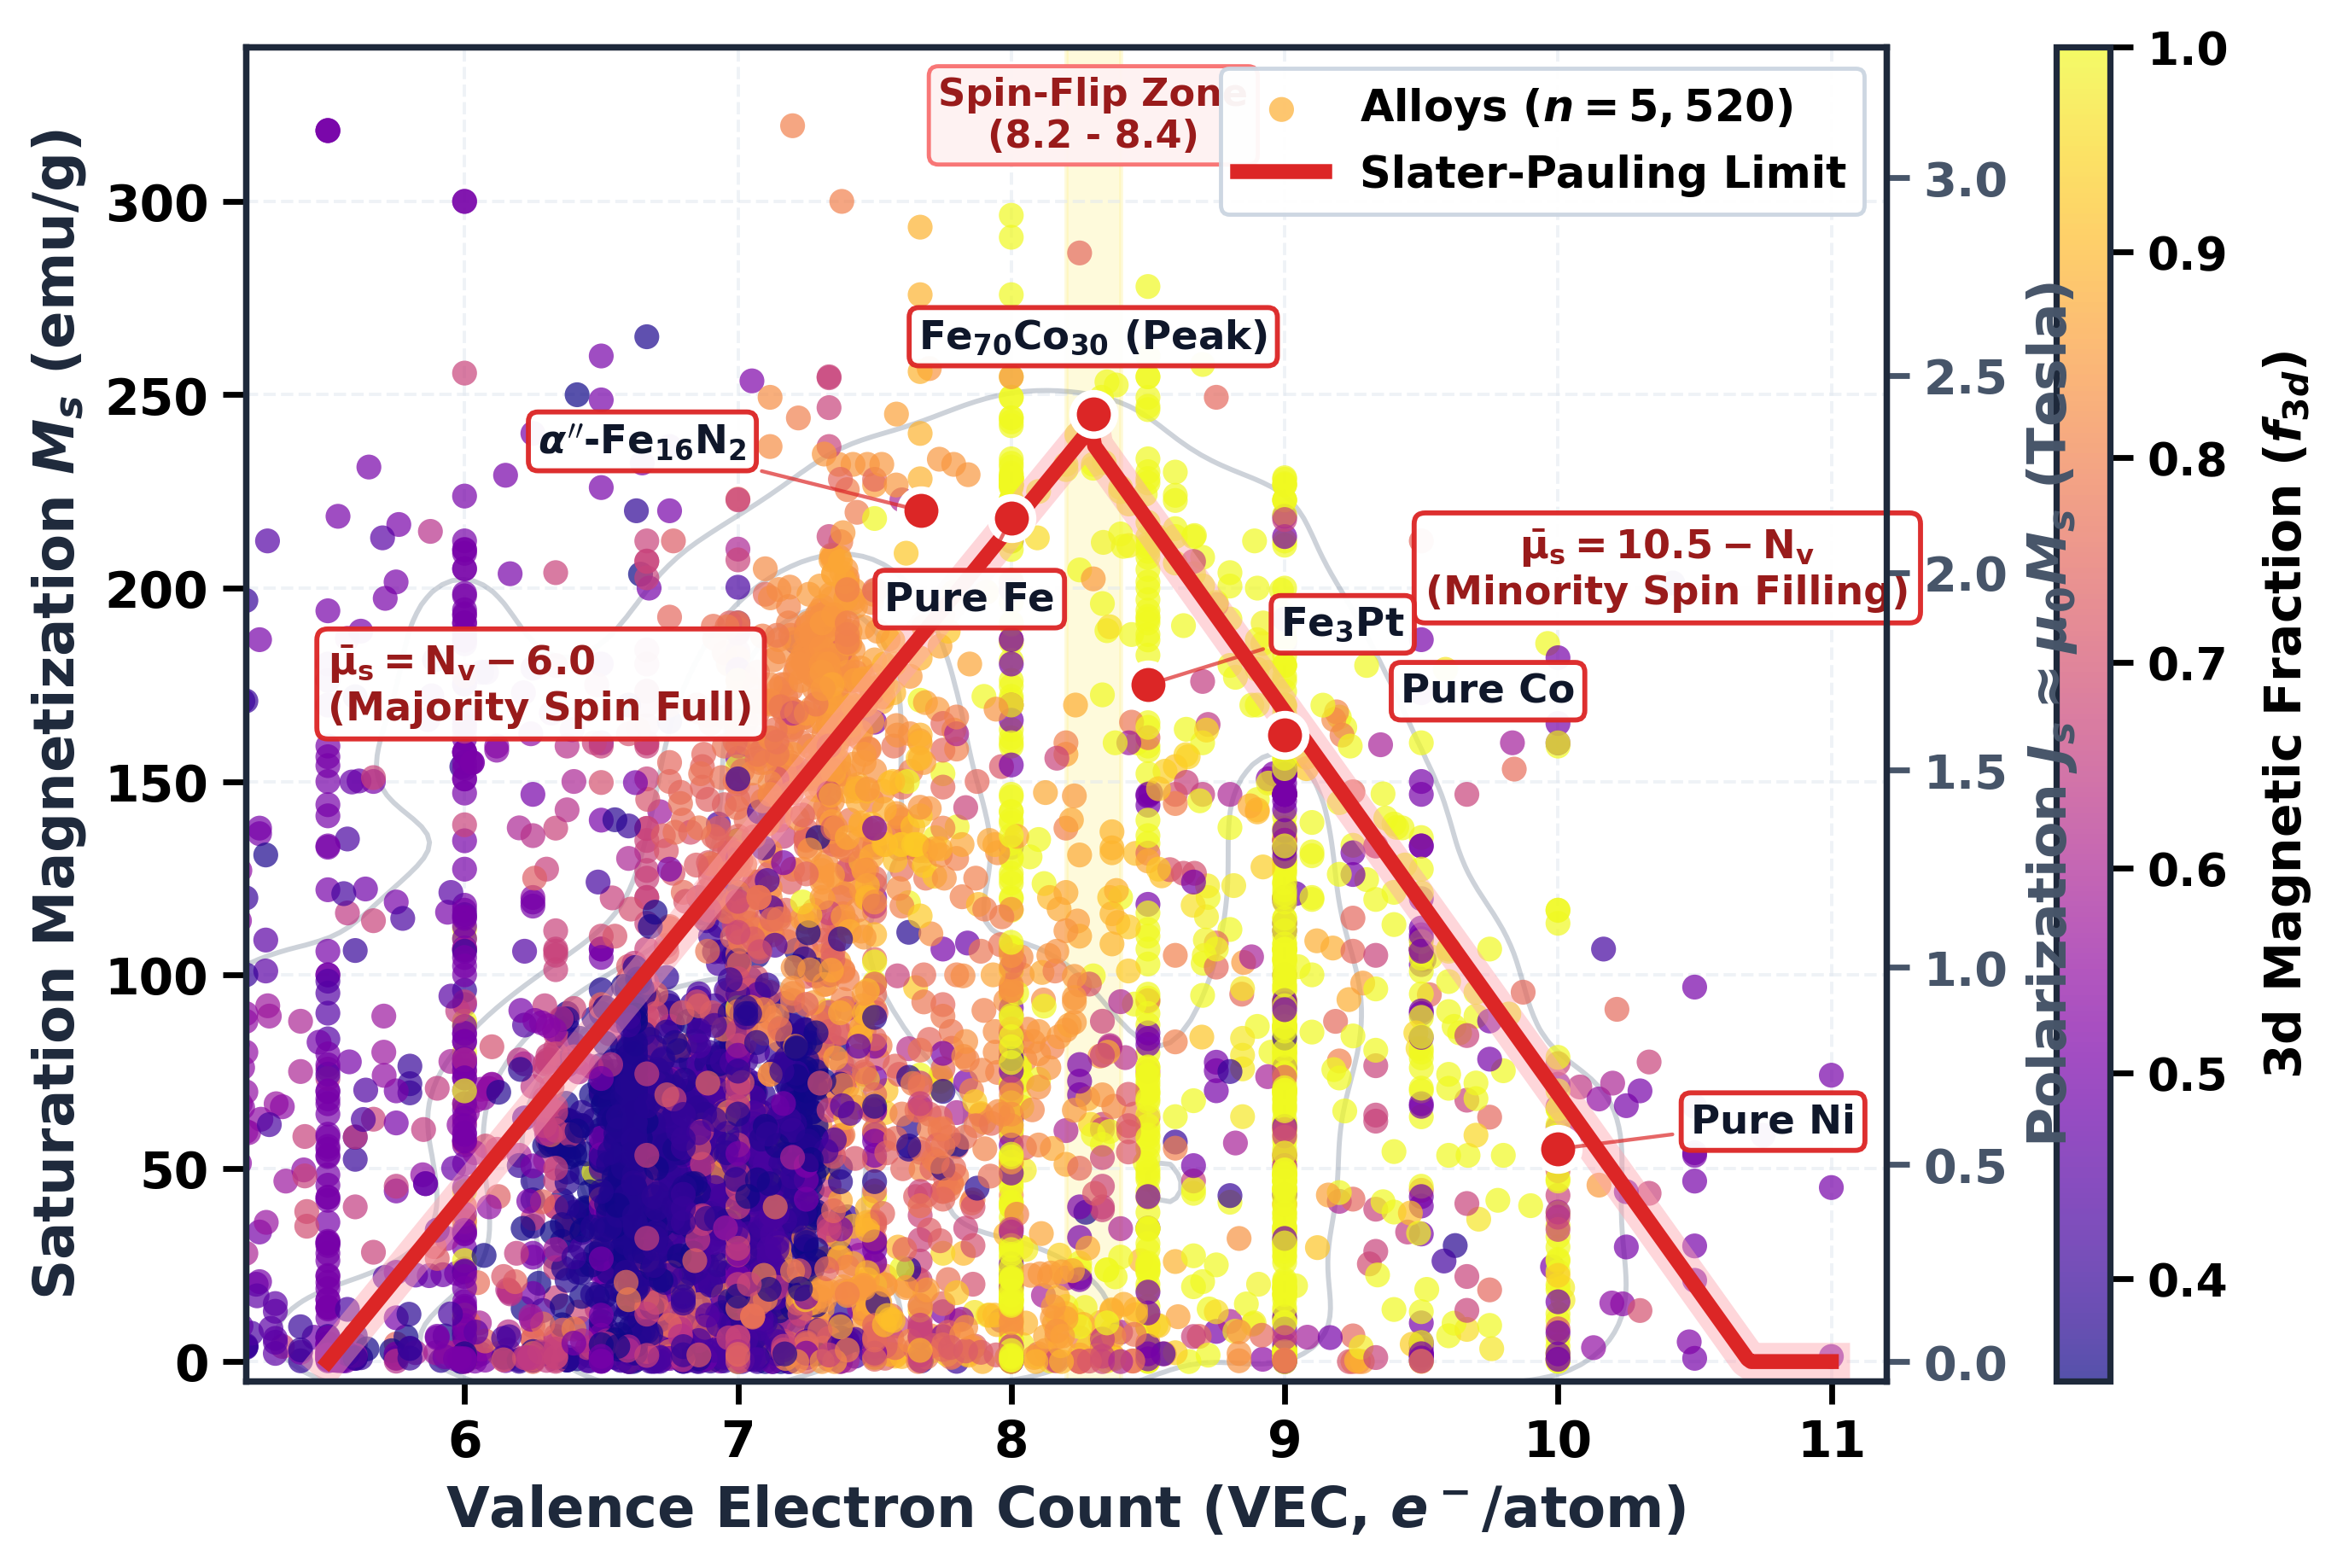
\includegraphics[height=4.7cm,keepaspectratio]{figures/slater_pauling_curve.png}
\vspace{-0.5em}
\caption{Measured saturation magnetization $M_s$ against valence electron concentration. The Slater-Pauling curve (red) is an upper boundary, not a fit: the data sits beneath it, peaking near $N_v \approx 8.25$ in Fe-Co.}
\label{fig:slater_pauling}
\end{figure}

\noindent\textbf{Band Saturation Limits and Experimental Scatter:}
Measured saturation magnetization peaks near $N_v \approx 8.25$--$8.40$ (Fe-Co), and the Slater-Pauling curve bounds the data from above across every alloy class (Figure~\ref{fig:slater_pauling}). Underneath that ceiling the scatter is wide---spin canting, ligand dilution in non-metallic phases and local crystal-field effects all reduce the moment, and none of them is visible in a composition. This is the key qualification on Table~\ref{tab:baselines}: the large Slater-Pauling MAE is not a failed prediction but the expected consequence of using a bound as if it were a regressor.

\noindent\textbf{Descriptor Correlation Drivers:}
Linear (Pearson $r$) and rank (Spearman $\rho$) dependencies between descriptors and magnetic properties (Figure~\ref{fig:correlations}) separate the physical drivers cleanly:

\begin{figure}[H]
\centering
\begin{subfigure}[b]{0.46\textwidth}
  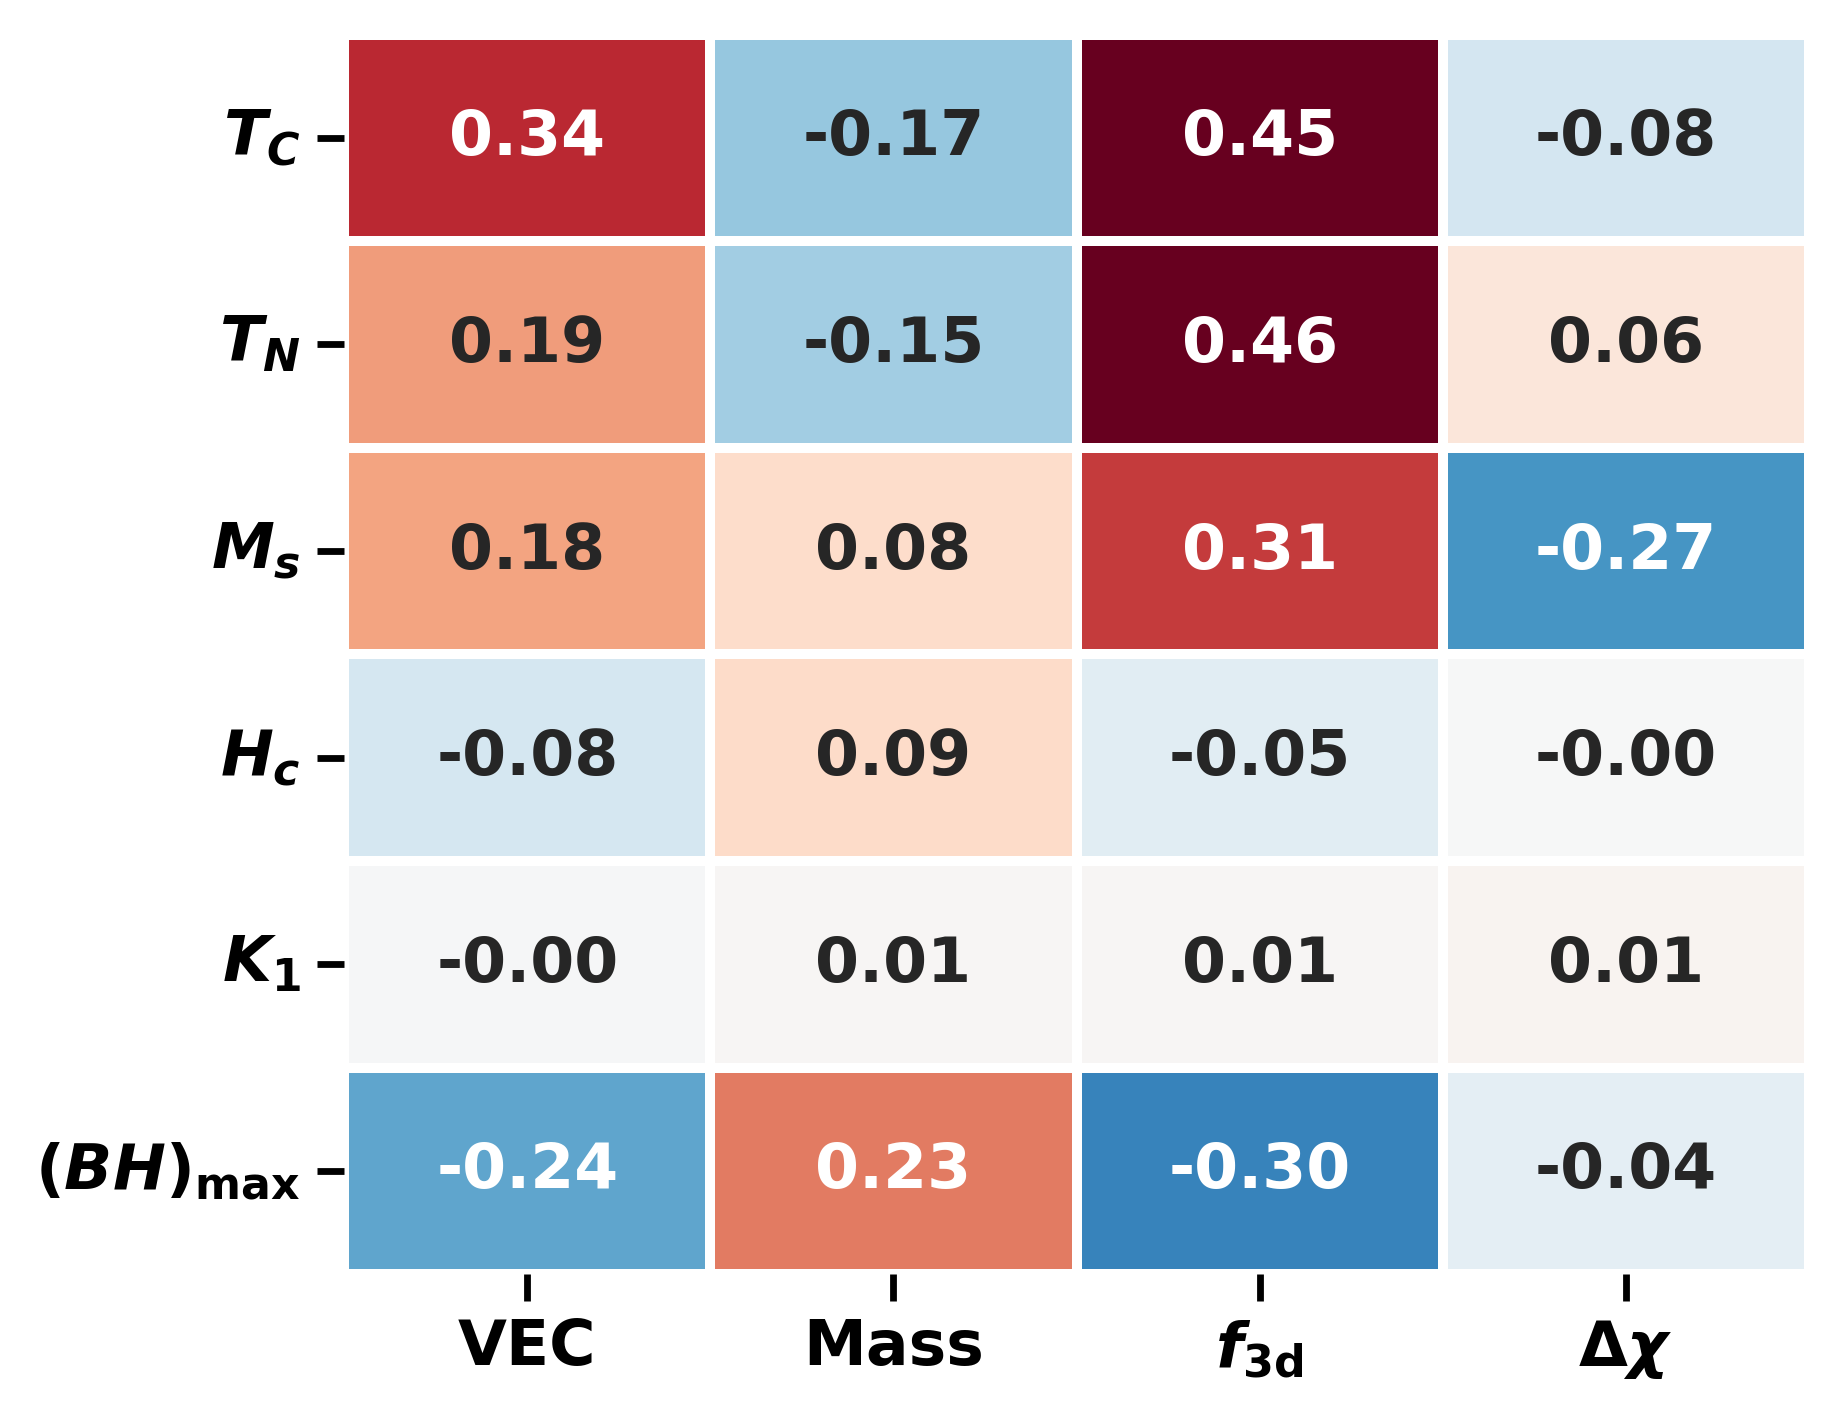
\includegraphics[width=\linewidth]{figures/corr_pearson.png}
  \caption{Pearson linear ($r$)}
  \label{subfig:pearson}
\end{subfigure}\hfill
\begin{subfigure}[b]{0.52\textwidth}
  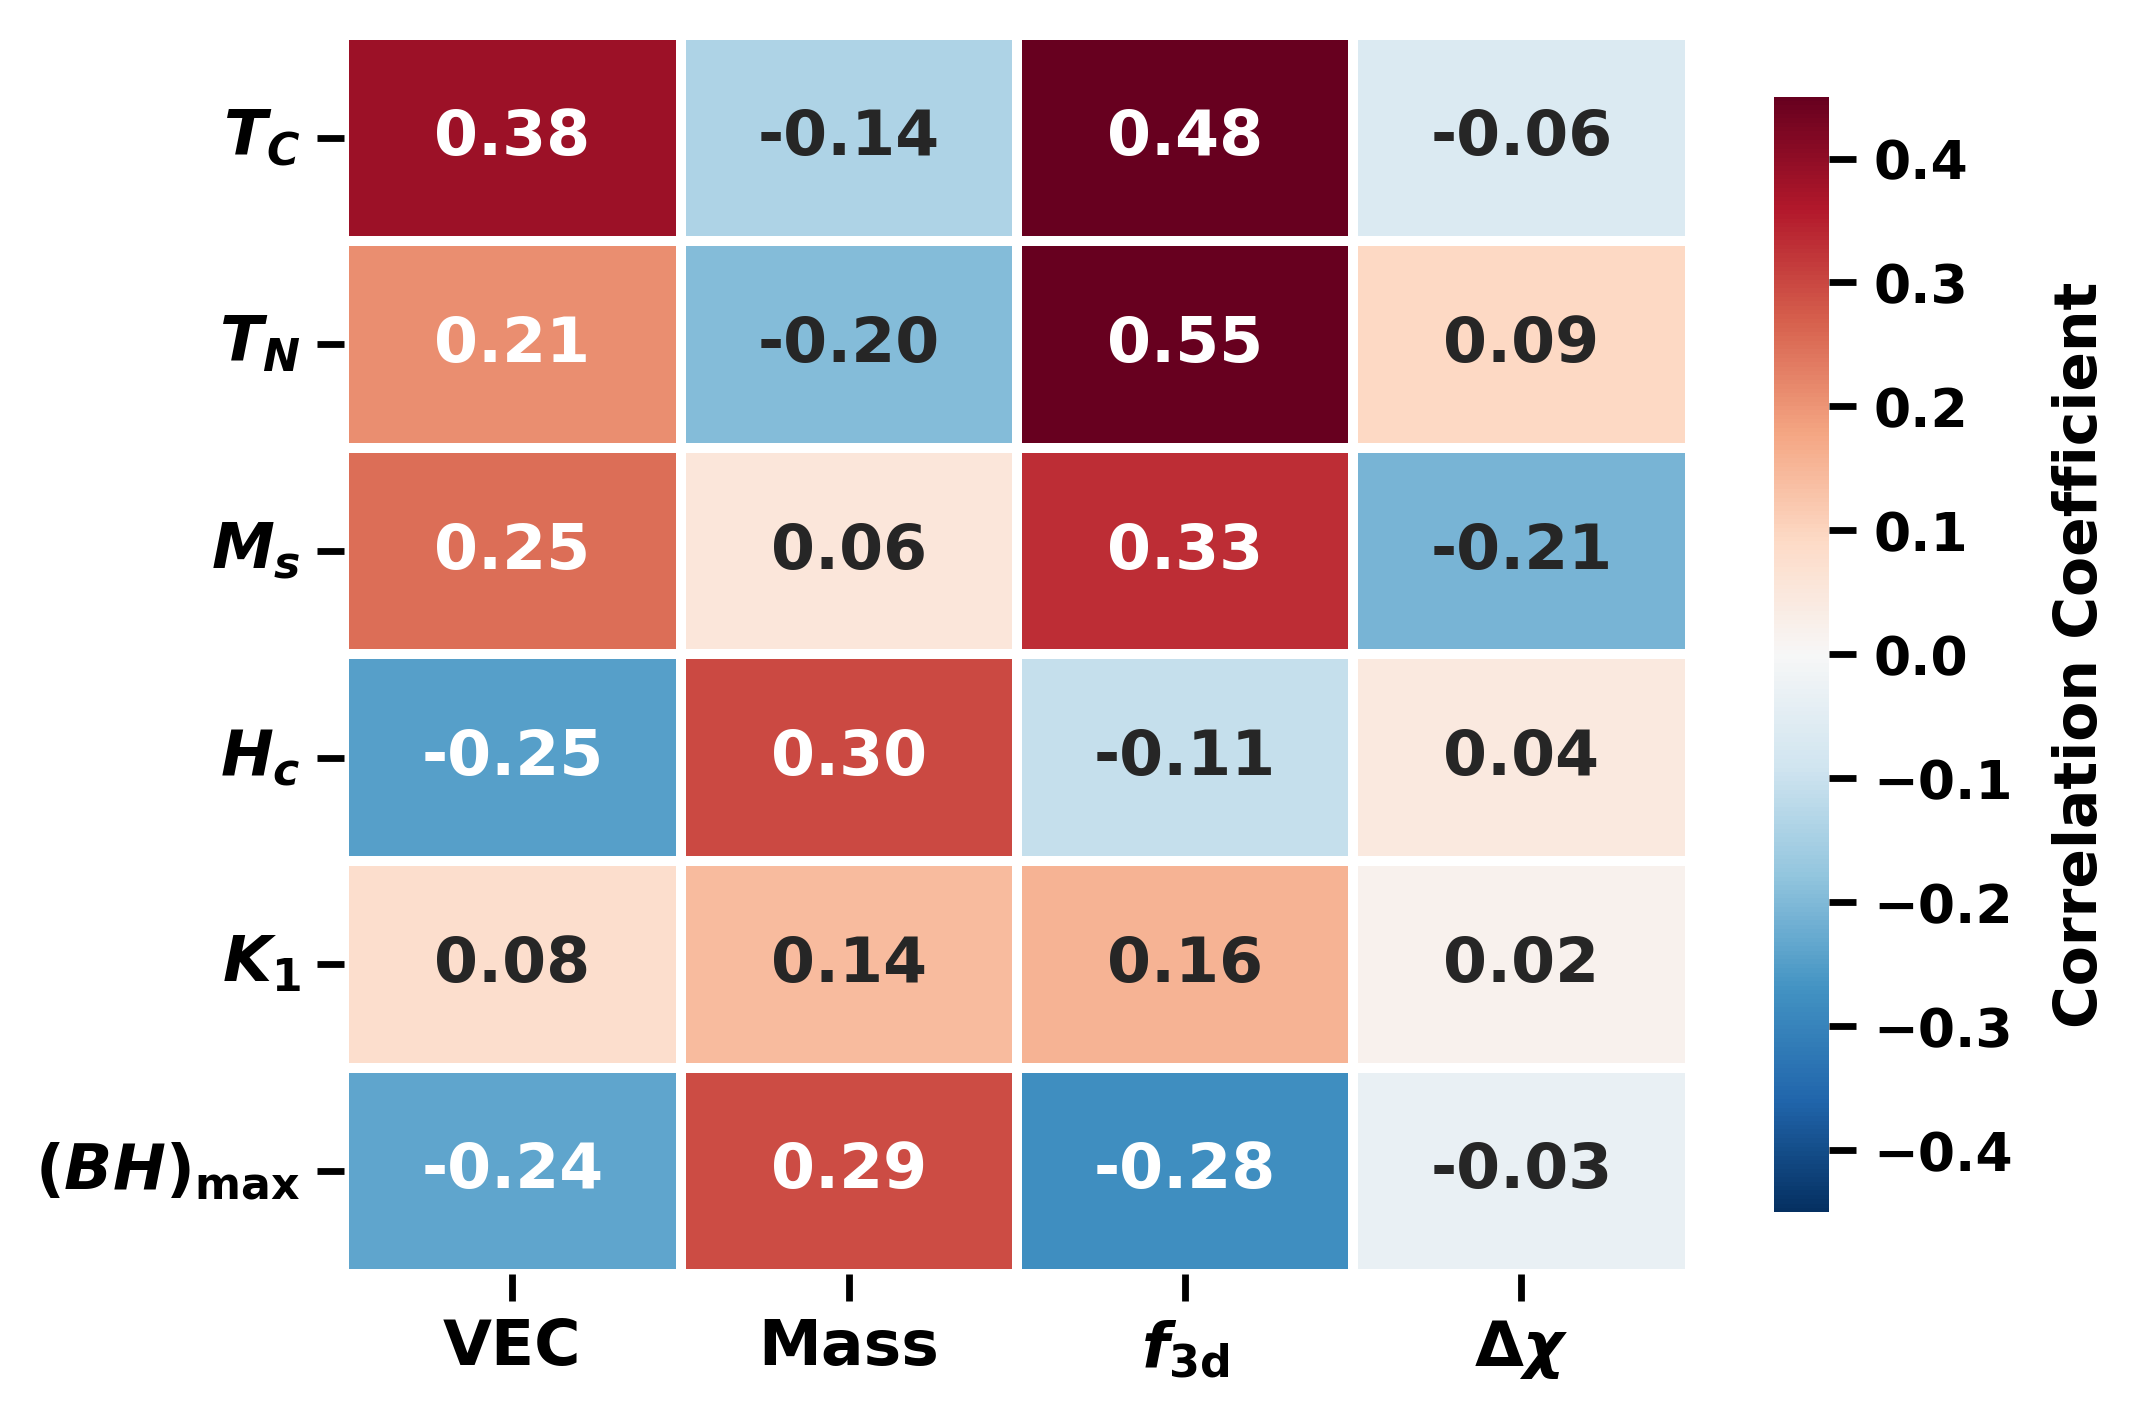
\includegraphics[width=\linewidth]{figures/corr_spearman.png}
  \caption{Spearman rank ($\rho$)}
  \label{subfig:spearman}
\end{subfigure}
\vspace{-0.4em}
\caption{Heatmaps of Pearson correlation $r$ (a) and Spearman rank correlation $\rho$ (b) between compositional descriptors and macroscopic magnetic properties, grouped from standalone visualizations.}
\label{fig:correlations}
\end{figure}

\noindent Key physical mechanisms identified from the correlation structure include:
\begin{itemize}
  \item \textbf{Rare-Earth Concentration ($f_{\text{RE}}$)}: Strongly drives coercive field and uniaxial magnetocrystalline anisotropy ($K_1$), governed by localized $4f$ electron shells with unquenched orbital angular momentum and strong spin-orbit coupling.
  \item \textbf{Transition-Metal Fraction ($f_{3d}$)}: Governs high Curie temperatures ($T_C$) and saturation magnetization ($M_s$) via direct interatomic $3d$--$3d$ quantum exchange coupling.
  \item \textbf{Valence Electron Count (VEC)}: Controls rigid-band filling, showing divergent trends between itinerant exchange ferromagnetism and defect-sensitive coercivity.
\end{itemize}

\clearpage
% =========================================================================
% Page 4
% =========================================================================

% =========================================================================
\section{Microstructural Defect Gap and Inverse Discovery Platform}
% =========================================================================
Intrinsic properties come close to their ceilings; coercivity does not. Figure~\ref{fig:kronmuller} compares measured $H_c$ against the ideal nucleation field $H_K$ for every record where $K_1$, $M_s$ and $H_c$ were all reported. The median polycrystal reaches $\alpha \approx 0.11$ of its own anisotropy limit. The remaining 89\% is lost to grain boundaries, misorientation and surface nucleation sites---and, decisively, none of those is a function of composition.

\begin{figure}[H]
\centering
\begin{subfigure}[b]{0.51\textwidth}
  \centering
  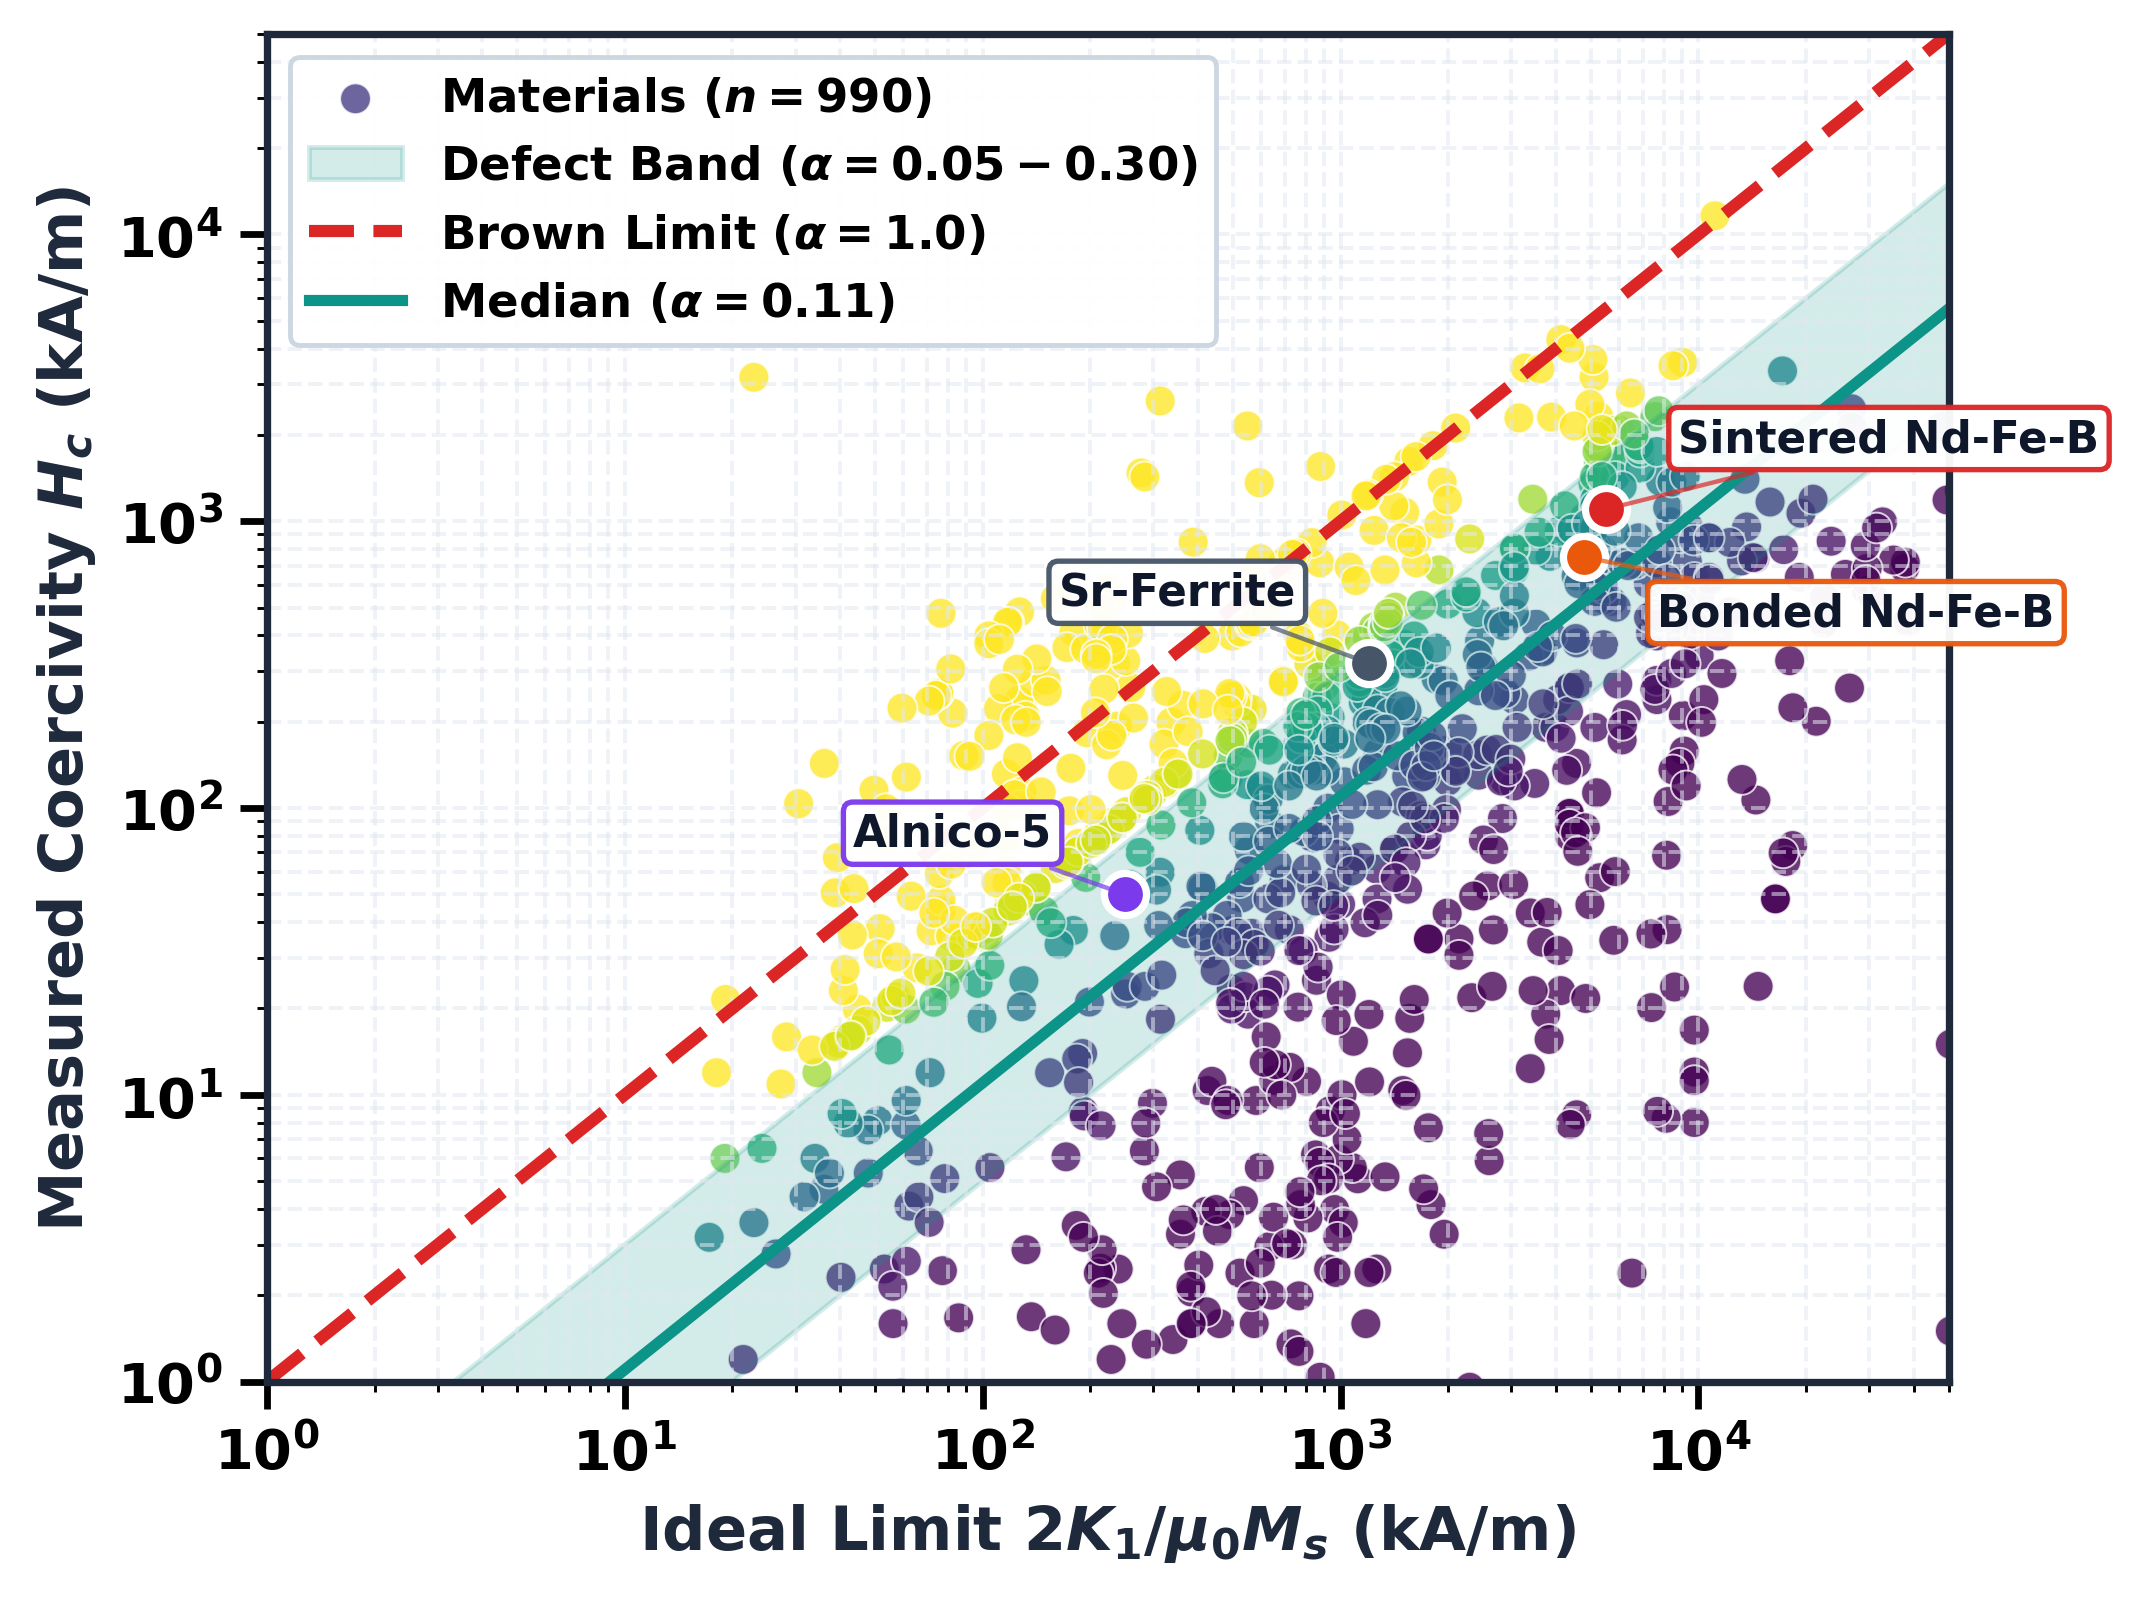
\includegraphics[height=3.85cm,keepaspectratio]{figures/kronmuller_scatter.png}
  \caption{Coercivity realization gap}
  \label{subfig:kron_scatter}
\end{subfigure}\hfill
\begin{subfigure}[b]{0.46\textwidth}
  \centering
  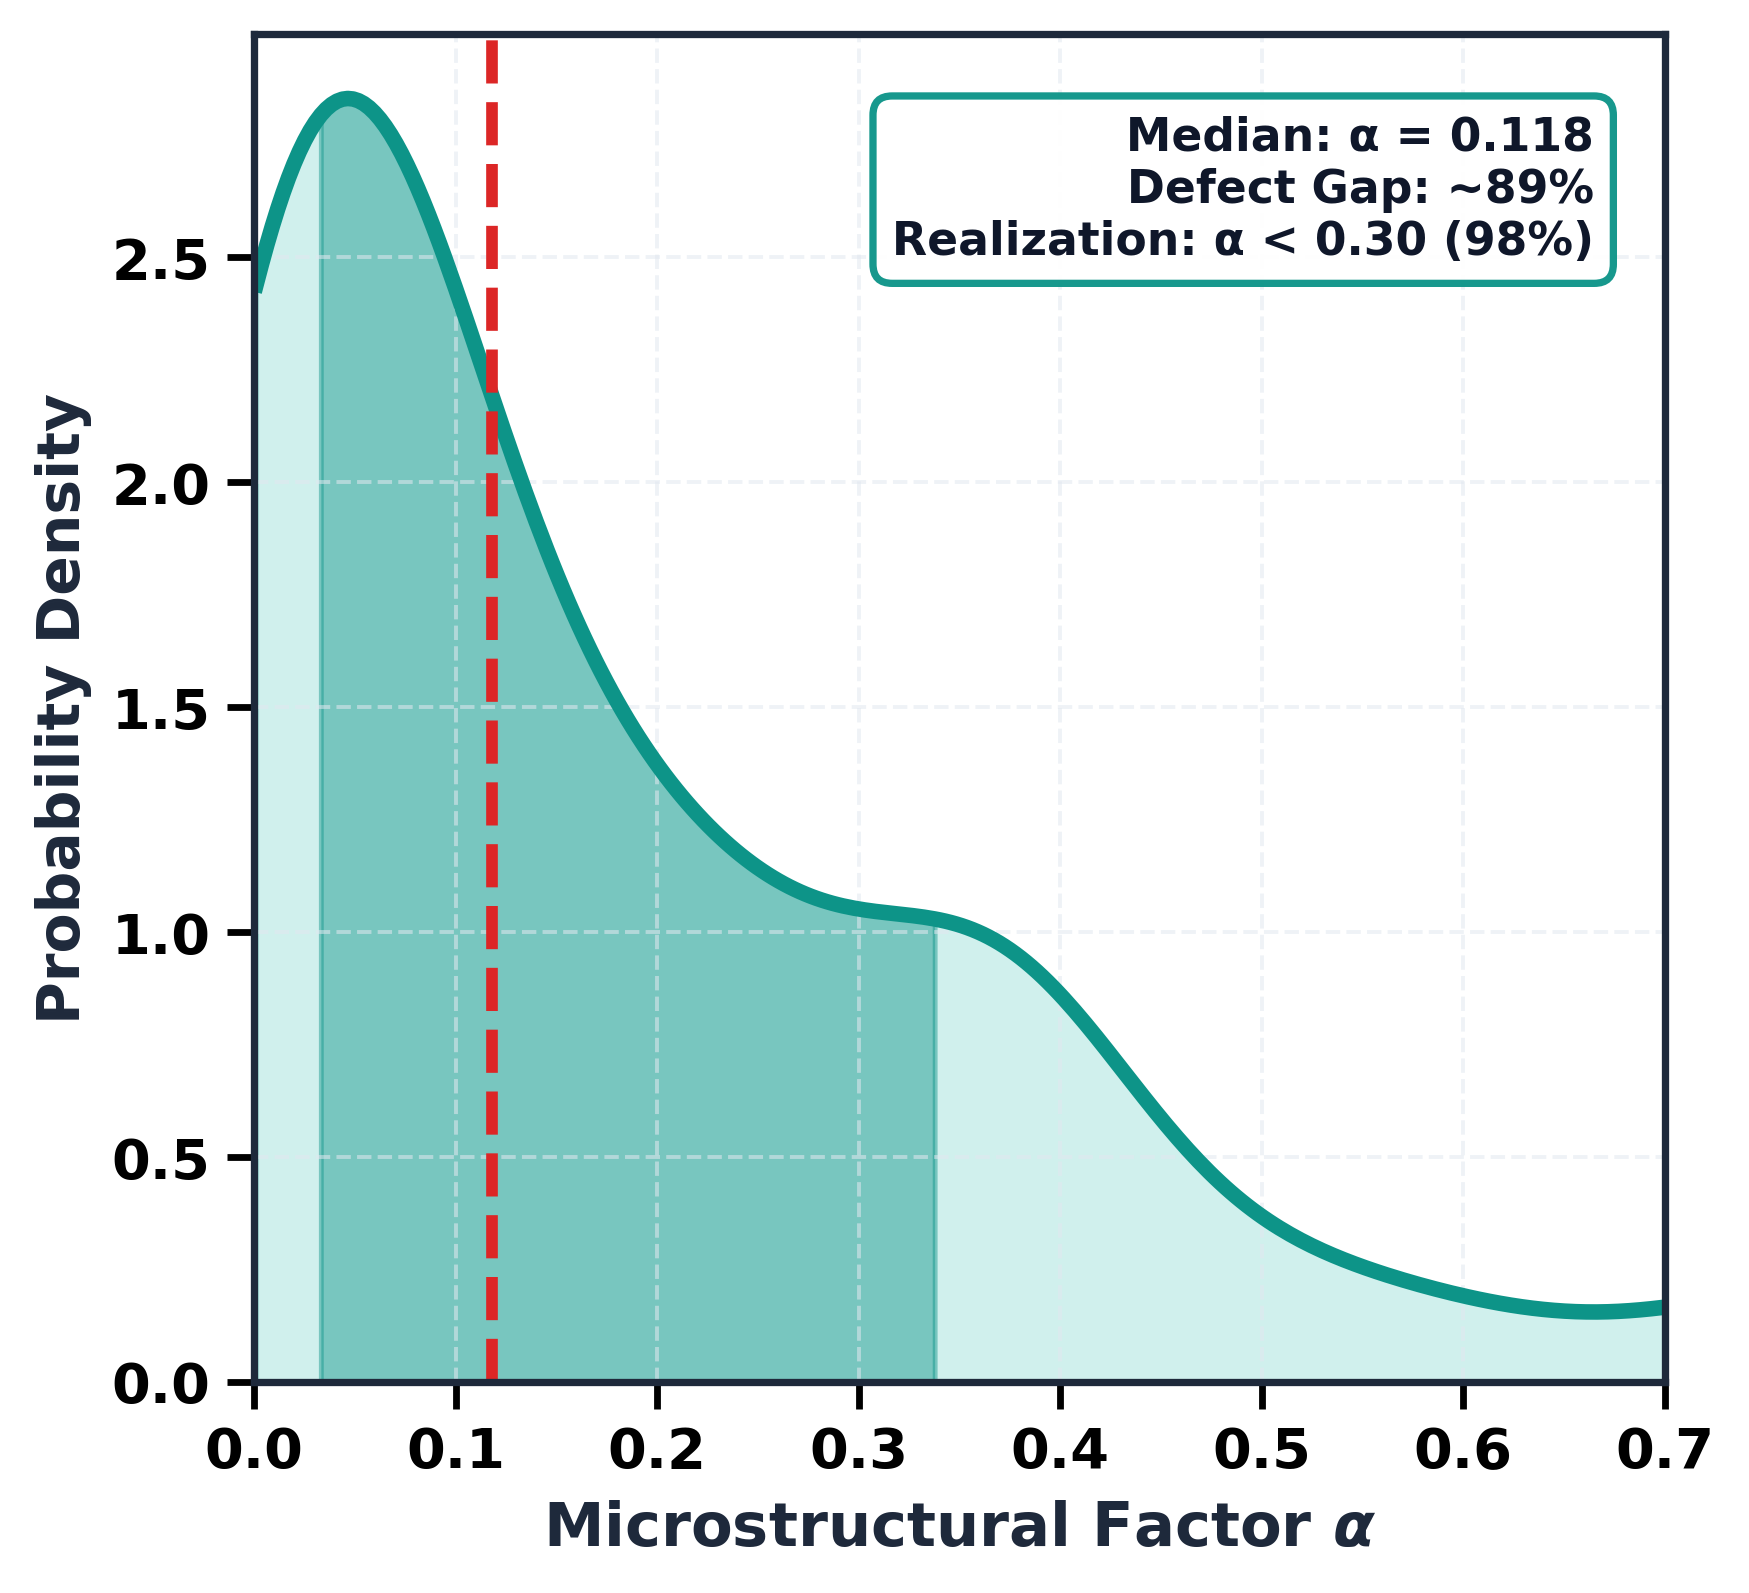
\includegraphics[height=3.85cm,keepaspectratio]{figures/kronmuller_defect_hist.png}
  \caption{Defect ratio ($\alpha = H_c / H_K$)}
  \label{subfig:kron_hist}
\end{subfigure}
\vspace{-0.5em}
\caption{Measured coercivity against the ideal Kronmüller ceiling $2K_1/\mu_0 M_s$: (a) the realization gap, with points falling one to two decades below the $\alpha = 1$ line, and (b) the distribution of $\alpha$, concentrated around a median of $0.11$.}
\label{fig:kronmuller}
\end{figure}
\vspace{-0.4em}

Closing this deficit requires 3D atomistic geometry rather than trial-and-error chemistry. We leverage two pretrained foundation models: \textbf{DAO} generates relaxed 3D crystal structures directly from stoichiometry and evaluates energy above the convex hull ($E_{\text{hull}}$) to eliminate thermodynamically unstable phases; \textbf{MACE} higher-order $E(3)$-equivariant message passing resolves polymorphic phase bifurcation (e.g., distinguishing ferromagnetic $\tau$-MnAl from paramagnetic $\beta$-MnAl sharing identical stoichiometry).

Downstream, a trained multi-task machine learning pipeline couples to these structural representations (Figure~\ref{fig:workflow}c). A trained classification ensemble (\texttt{phase\_clf}, 91.9\% accuracy, 0.908 macro $F_1$) predicts ground-state ordering (FM, AFM, NM), dynamically routing to dedicated regressors: Curie temperature $T_C$ ($R^2 = 0.816$) for ferromagnetic systems and Néel temperature $T_N$ ($R^2 = 0.741$) for antiferromagnetic systems, alongside trained models for $M_s$, $H_c$, $K_1$, and $(BH)_{\max}$ with 90\% conformal bounds. An inverse discovery engine screens rare-earth-free candidates satisfying $(BH)_{\max} \ge 120$~kJ/m$^3$ and $T_C \ge 450$~K, re-checked against fundamental ceilings. The companion open-source application (Figure~\ref{fig:app_screenshot}) provides real-time bound calculation, 3D unit cell generation, and gap diagnostics.

\begin{figure}[H]
\centering
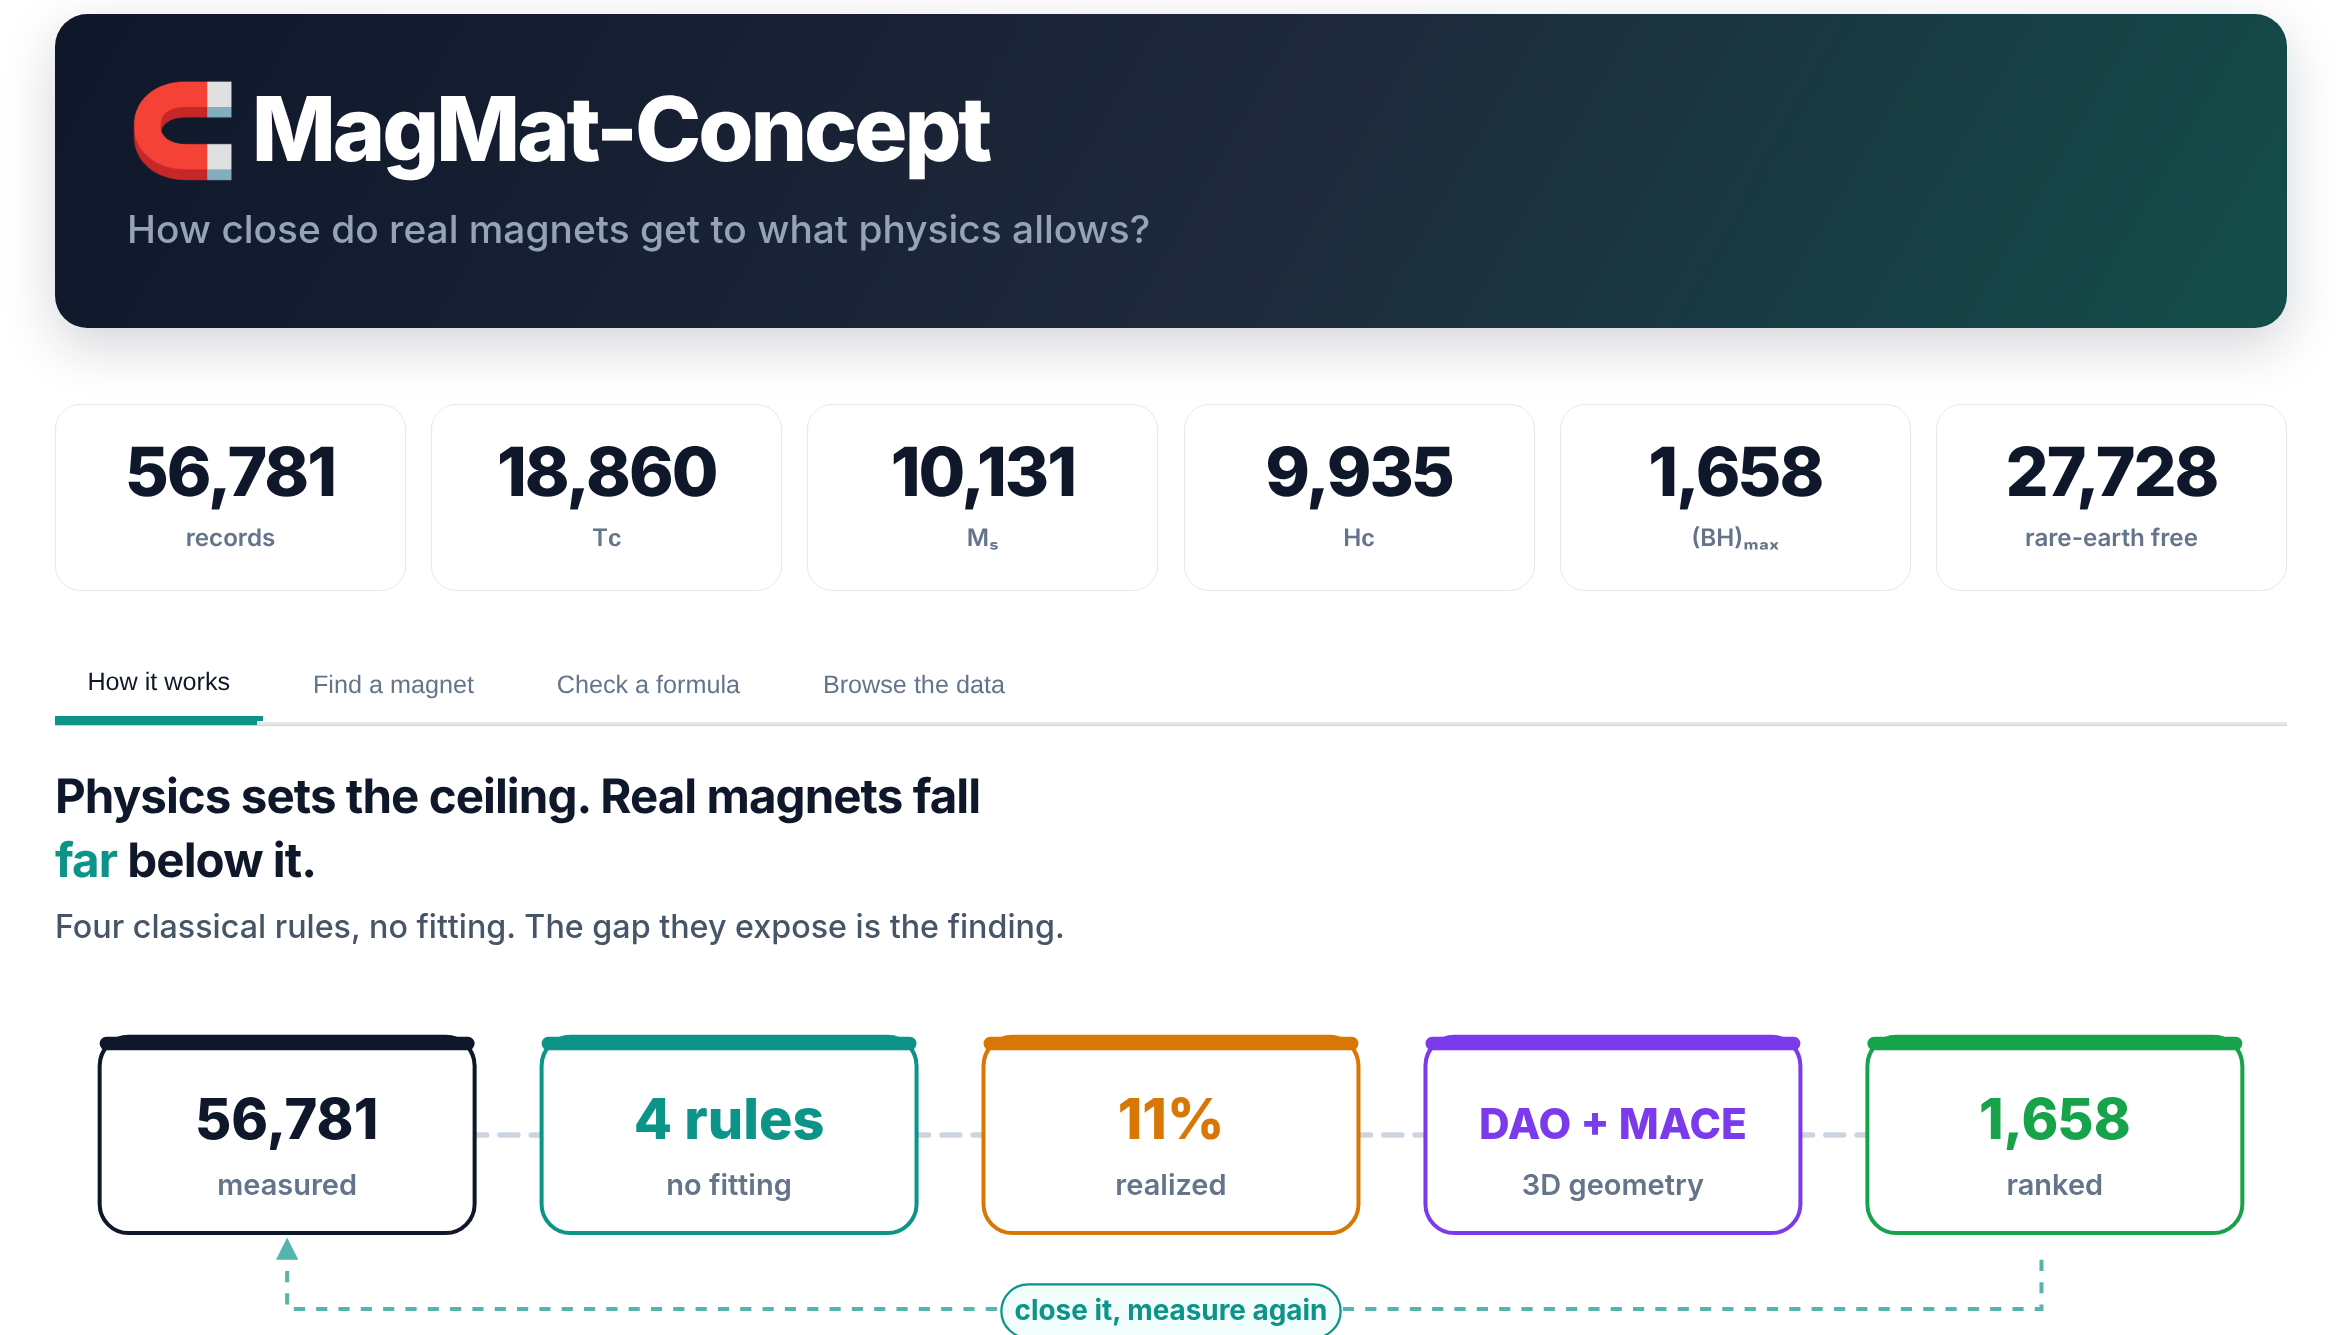
\includegraphics[width=\linewidth,height=4.6cm,keepaspectratio]{figures/simple_app_screenshot.png}
\vspace{-0.5em}
\caption{The open-source Streamlit application: an animated schematic of the four bounds and the gap between them, a physics calculator for any composition, and candidate ranking against user-defined $(BH)_{\max}$ and $T_C$ targets.}
\label{fig:app_screenshot}
\end{figure}
\vspace{-0.4em}

% =========================================================================
\section{Conclusions}
% =========================================================================
Four classical rules, applied to 56,781 records and fitted to nothing, give a clear division of labour. Magnetization is already near its atomic ceiling ($M_s \approx 245$~emu/g), and the Maxwell bound holds for 71.7\% of matched records while flagging the rest as inconsistent data. Coercivity is the outlier: the median magnet reaches only $\alpha \approx 0.11$ of its own anisotropy limit. That 89\% shortfall is governed by microstructure rather than chemistry, so it is precisely the part a compositional model cannot learn---which is the argument for 3D structural descriptors (DAO, MACE) and the predictors built on them. Establishing the bounds first makes that argument quantitative rather than assumed.
\vspace{-0.4em}

% =========================================================================
\section*{References}
% =========================================================================
\begingroup
\footnotesize
\begin{enumerate}[label={[\arabic*]}, leftmargin=1.5em, itemsep=-3pt, topsep=1pt]
  \item J.~M.~D.~Coey, \emph{Magnetism and Magnetic Materials}, Cambridge University Press, 2010.
  \item H.~Kronmüller, \emph{Micromagnetism of High-Technology Permanent Magnets}, J. Magn. Magn. Mater., \textbf{7}, 341, 1987.
  \item J.~Slater, \emph{The Ferromagnetism of Nickel. II}, Phys. Rev., \textbf{49}, 537, 1936; L.~Pauling, Phys. Rev., \textbf{54}, 899, 1938.
  \item I.~Batatia \emph{et al.}, \emph{MACE: Higher Order Equivariant Message Passing Neural Networks}, NeurIPS, \textbf{35}, 11423, 2022.
  \item DAO Framework, \emph{Diffusion for Atomistic Ordering and Crystal Structure Generation}, 2026.
\end{enumerate}
\endgroup

\end{document}
